\documentclass[12pt, twoside]{book}

% Elenco dei packages utilizzati
\usepackage[a4paper,width=150mm,top=25mm,bottom=25mm,bindingoffset=6mm]{geometry}
\usepackage[utf8]{inputenc}
\usepackage[T1]{fontenc}
\usepackage[italian]{babel}
\usepackage{subcaption}
\usepackage{graphicx}
\usepackage{fancyhdr}
\usepackage{float}
\usepackage{color}
\usepackage[nottoc]{tocbibind}
\usepackage{emptypage}
\usepackage[hidelinks]{hyperref}
\usepackage{titlesec}
\usepackage{amssymb}
\usepackage[sorting=none,backend=bibtex]{biblatex}
\usepackage{csquotes}
\usepackage{pdfpages}
\usepackage{amsmath}
\usepackage{placeins}
\usepackage{hyperref}
\usepackage{footnote}
\usepackage{import}

% \usepackage{minted}
\usepackage{xcolor}

% page styles
\pagestyle{fancy}
\definecolor{LightGray}{gray}{0.9}
\setlength{\parindent}{0em}
\setlength{\parskip}{0.5em}

% \usemintedstyle{colorful}

% Bibliography
\addbibresource{./bibliography/bibliography.bib}

\begin{document}

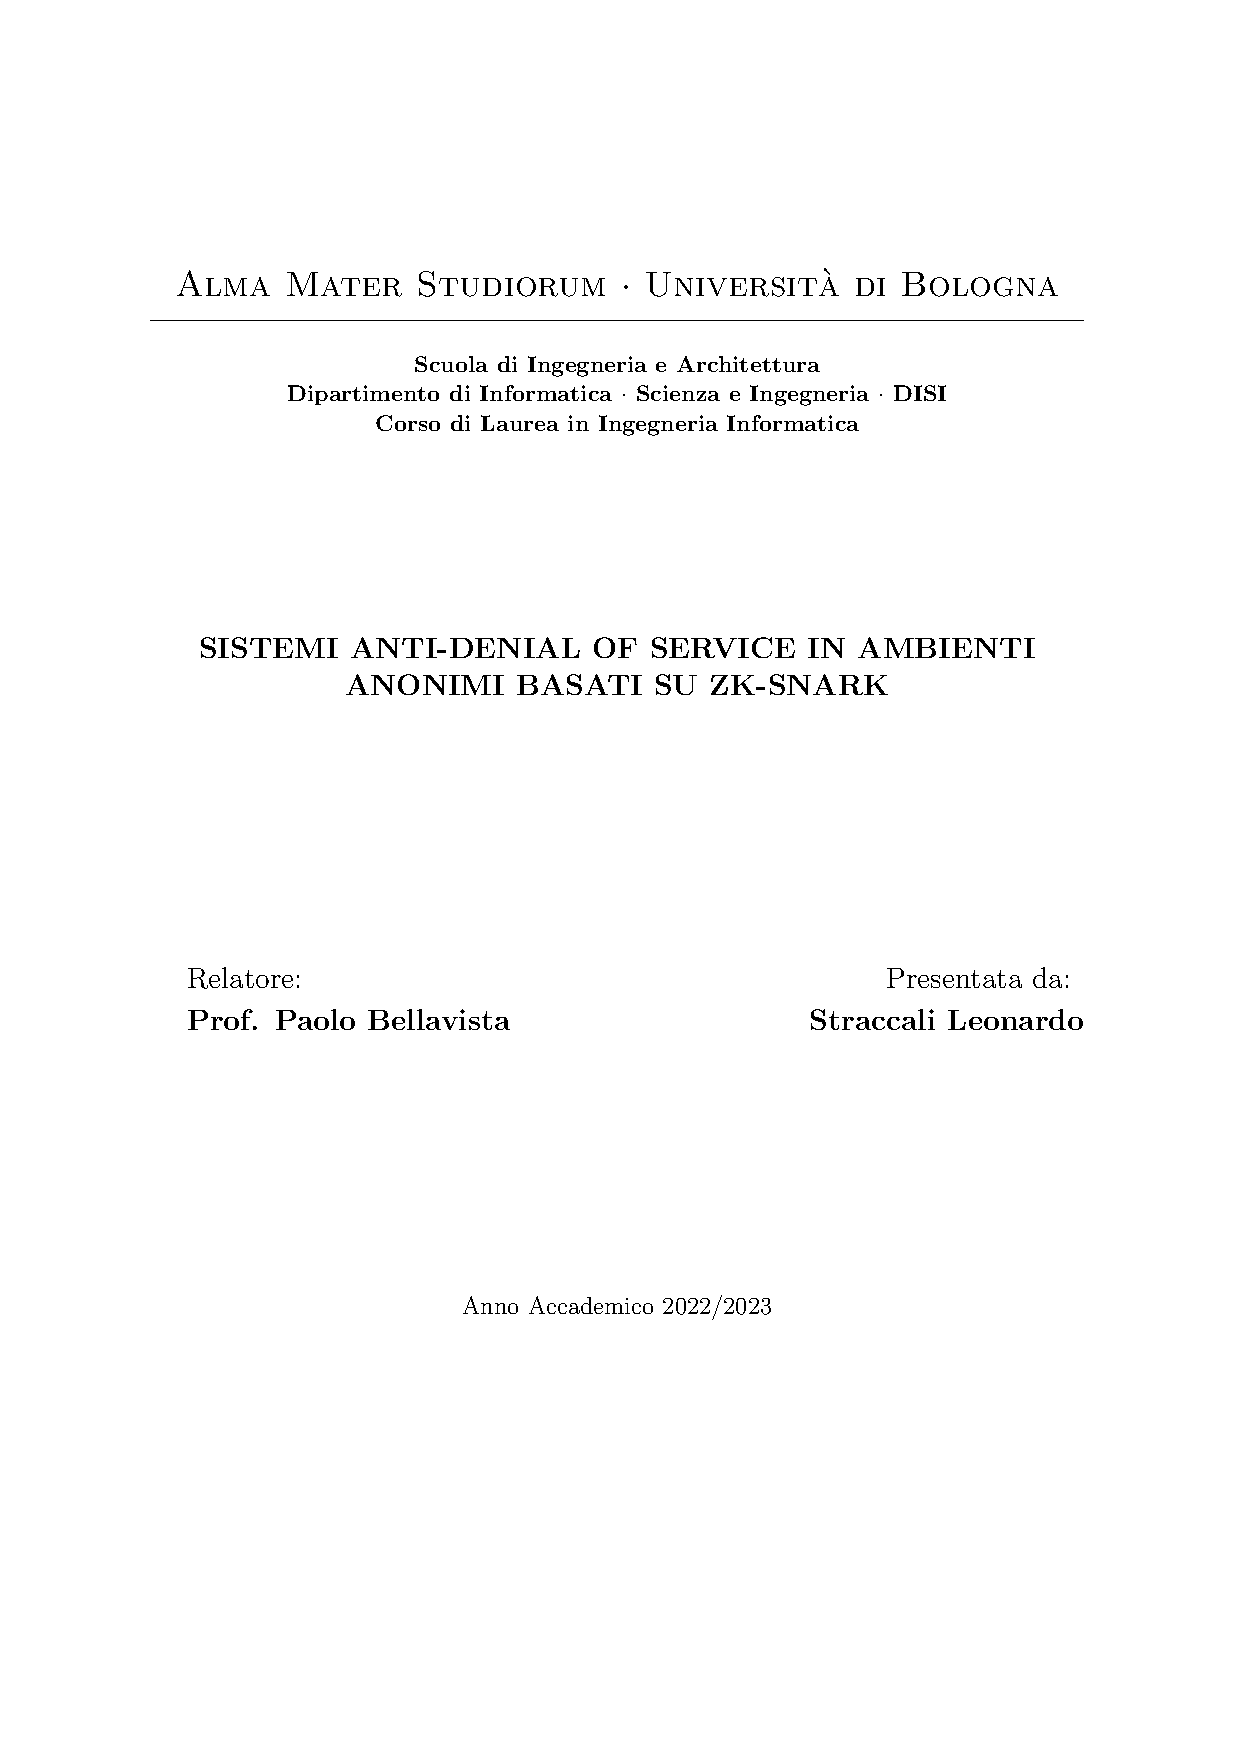
\includepdf{chapters/0.frontpage/front.pdf}

\cleardoublepage
\begin{flushright}
\thispagestyle{empty}
\null\vspace{\stretch {1}}
\textit{
    “\break
    \break
    ”
    \break ---.}
\vspace{\stretch{2}}\null
\end{flushright}
\cleardoublepage

\tableofcontents

\phantomsection
\listoffigures

\chapter*{Introduzione}
\chaptermark{Introduzione}
\addcontentsline{toc}{chapter}{Introduzione}
\label{chap:introduction}

L’implementazione di strumenti atti a combattere gli attacchi di tipo \textbf{denial of service}, sono da molto
tempo materia di studio e di ricerca. Questi attacchi possono rappresentare una minaccia grave, soprattutto quando si
verificano su servizi cruciali e sensibili. Per tale motivo, negli anni sono state sviluppate molte strategie diverse
per impedire a singoli o ai gruppi di computer (noti anche come "zombie armies") di attaccare servizi o reti.
Attualmente una delle metodologie di protezione più comuni agli attacchi \textbf{DoS} è il \textbf{Rate-limiting}, che permette
di imporre una frequenza massima accettabile per le richieste, al fine di evitare sovraccarichi e congestionamenti delle
risorse. In particolare, nei sistemi su larga scala, la limitazione della frequenza rappresenta uno strumento essenziale
per garantire la disponibilità e l'integrità delle risorse e dei servizi.

Un altro campo di interesse in cui si sono fatti molti progressi negli ultimi anni, grazie soprattutto all'avvento delle
tecnologie blockchain, è stato quello dell’anonimato in rete. Con il termine anonimato in rete ci si riferisce alla
condizione in cui, sulla base di una conoscenza parziale o totale delle interazioni di un utente in una rete, non è
possibile risalire all'identità dell'utente stesso; permettendo un'interazione con i servizi offerti dalla rete in
assoluta riservatezza. L'anonimato in rete presenta molteplici vantaggi, soprattutto in contesti in cui la privacy
costituisce un requisito fondamentale, come ad esempio nelle votazioni o nelle transazioni finanziarie. Inoltre, la
possibilità di mantenere l'anonimato può rivelarsi altrettanto utile in ambiti più diffusi, come le conversazioni online
o i social network, garantendo la libertà di espressione e la tutela della propria sfera privata.

Tuttavia, l'anonimato in rete presenta anche alcune criticità, tra cui la principale è rappresentata dalla difficoltà di
controllo. La ragione di questa difficoltà è da individuare nel fatto che le metodologie di sicurezza a livello applicazione (pila ISO/OSI)
generalmente si basano sull' analisi del comportamento degli utenti o dei dispositivi, nel corso del tempo, al
fine di rilevare i pattern di attività che potrebbero suggerire la presenza di un attacco. In un contesto anonimo, in
cui le identità degli utenti non sono tracciabili, ciò diviene notevolmente più arduo. Esistono strumenti di
rate-limiting efficaci a livelli inferiori della pila ISO/OSI, come a livello di trasporto o di sessione. Tuttavia, la
loro attuazione comporta alcuni svantaggi, come il rischio di limitare o bloccare numerosi indirizzi IP tradotti sotto
una NAT, minare la privacy degli utenti disattivando protezioni utili come TLS o ancora essere elusi da
tecniche di mascheramento, come l'IP spoofing. Per tali motivazioni, per un servizio diffuso in ambiente anonimo, non è
possibile fare affidamento esclusivamente su questi strumenti.
\clearpage
La presente tesi affronta la discussione di un protocollo chiamato \textbf{RLN (Rate-Limiting Nullifier)}\footnote{\url{https://rate-limiting-nullifier.github.io/rln-docs/}} basato sulla tecnologia
\textbf{zk-SNARK}, che permette di attuare un rate-limiting in ambiente anonimo. Il protocollo è composto da tre parti generali,
le quali si differenziano, nei dettagli, a seconda del dominio applicativo.
Fasi del protocollo:
\begin{itemize}
    \item \textbf{Registrazione}: Durante questa fase, gli utenti che desiderano accedere al servizio devono
    registrarsi fornendo una prova del possesso di determinati requisiti. Questa prova di possesso è denominata
    "identity commitment" e viene conservata e utilizzata nelle fasi successive del protocollo. I dati personali che
    soddisfano i requisiti sono definiti "stake" e possono assumere forme diverse a seconda del contesto applicativo. Ad
    esempio, possono essere costituiti da un profilo su un social network, dall'indirizzo di un portafoglio di
    criptovalute o da un'identità digitale come lo SPID o la CIE.

    Gli stake non vengono conservati dal protocollo. Alla fine della fase di registrazione, il sistma è a conoscenza
    unicamente nel fatto che un nuovo utente anonimo che soddisfa le specifiche della registrazione è
    stato aggiunto al servizio. La presenza di uno stake non è strettamente necessaria per la registrazione.
    In effetti, è possibile registrarsi semplicemente creando un codice univoco e fornendolo come identity commitment.
    Tuttavia, l'utilizzo di uno stake risulta essere molto utile al fine di prevenire attacchi Sybil, ovvero la
    generazione di numerosi utenti malevoli da parte di un attaccante.
    \item \textbf{Interazione}: Dopo essersi registrati, gli utenti hanno la possibilità di interagire con il servizio
    attraverso l'invio di richieste. Ad ogni richiesta, gli utenti sono tenuti a fornire una prova di appartenenza al
    sistema. Tale prova è generata tramite la tecnologia zk-SNARK, che consente di dimostrare al servizio che l'utente è
    effettivamente un membro legittimo senza rivelare alcuna informazione sulla sua identità. Inoltre, il protocollo
    consente di implementare una regola di rate-limiting, che, se non rispettata, porta l'utente a rivelare la propria
    stake. Ciò consente di scoprire e gestire chi attua comportamenti di spam o Dos, e di procedere alla fase
    successiva.
    \item \textbf{Punizione}: La tipologia e il grado di punizione dipendono molto dal contesto applicativo. Ad esempio,
    alcune punizioni o misure di "slashing" possono comportare la rimozione del membro dal gruppo, con conseguente
    impossibilità di interagire con il sistema e perdita dell'anonimato. In presenza di una stake, è possibile
    prevedere sanzioni più articolate, come l'inserimento dell'identità virtuale in un registro di esclusione per altri
    servizi, o la rivelazione dell'indirizzo del portafoglio criptovalute dell'utente e il sequestro dei fondi.
\end{itemize}
Di seguito si cercherà di guardare a tutto tondo le tecnologie e le idee alla base di zk-SNARK e del protocollo RLN.
Inoltre si mostrerà l'implementazione di un piccolo prototipo che utilizza questo protocollo per evitare il sovraccarico
di risorse in un servizio basato su API.
\clearpage
\chapter{Stato dell’arte}
\chaptermark{Stato dell’arte}
\label{chap:state-of-art}

\section{Denial-of-Service (DoS)}

Gli attacchi di tipo Denial-of-Service (DoS) sono una tipologia di attacchi informatici estremamente diffusi, la cui
frequenza è cresciuta negli anni sia in termini quantitativi che qualitativi. Questo incremento è stato determinato
dalla relativa facilità con cui è possibile condurre un attacco di questo tipo, nonché dalle sue conseguenze, che in
base alle contromisure adottate e alla struttura del servizio attaccato possono essere più o meno gravi. Nella tesi ci
concentreremo solamente, sull’analisi della metodologia di protezione denominate rate-limiting. Queste strategie possono
risultare estremamente efficaci in alcune situazioni, come dimostrato dall’evento accaduto ad agosto 2022 a Google \cite{google_ddos},
la quale grazie all’attivazione di un rate-limiter è stata in grado di contrastare con successo il più grande attacco di tipo
DDoS a livello applicativo mai registrato. Tale attacco, proveniente da oltre 5.256 sorgenti IP dislocate in 132 paesi
differenti, ha raggiunto il picco di 46 milioni di richieste al secondo. 

In generale, un una regola per il rate-limiting consiste in un semplice conteggio delle occorrenze delle richieste in un
lasso di tempo. Tuttavia, esistono diverse tecniche per misurare e limitare la frequenza di tali richieste, ognuna con i
propri usi e implicazioni.
\begin{itemize}
    \item \textbf{Fixed window}: Tra tutte le strategie che vedremo è la più semplice da implementare, consiste nello stabilire un
    limite massimo al numero di richieste che possono essere inviate in un determinato intervallo di tempo, detto
    "finestra". Ad esempio, si potrebbe limitare il numero di richieste a 100 ogni minuto. Questo limite viene applicato in
    modo uniforme all'interno della finestra temporale. Ciò significa che, una volta raggiunto il limite massimo di
    richieste consentite, l'utente o l'applicazione deve attendere il termine della finestra temporale per poter inviare
    nuove richieste. Uno svantaggio significativo di questa strategia è la possibile concentrazione di richieste tutte in
    una porzione della finestra, rischiando un sovraccarico del servizio. Caso notevole è il caso in cui si concentrino tutte
    le richieste di una finestra al margine della fine e tutte le richieste della finestra successiva al margine dell’inizio
    questo comporta che il sistema in una durata equivalente a quella della finestra gestisca il doppio delle richieste
    consentite.
    \begin{figure}[H]
        \centering
        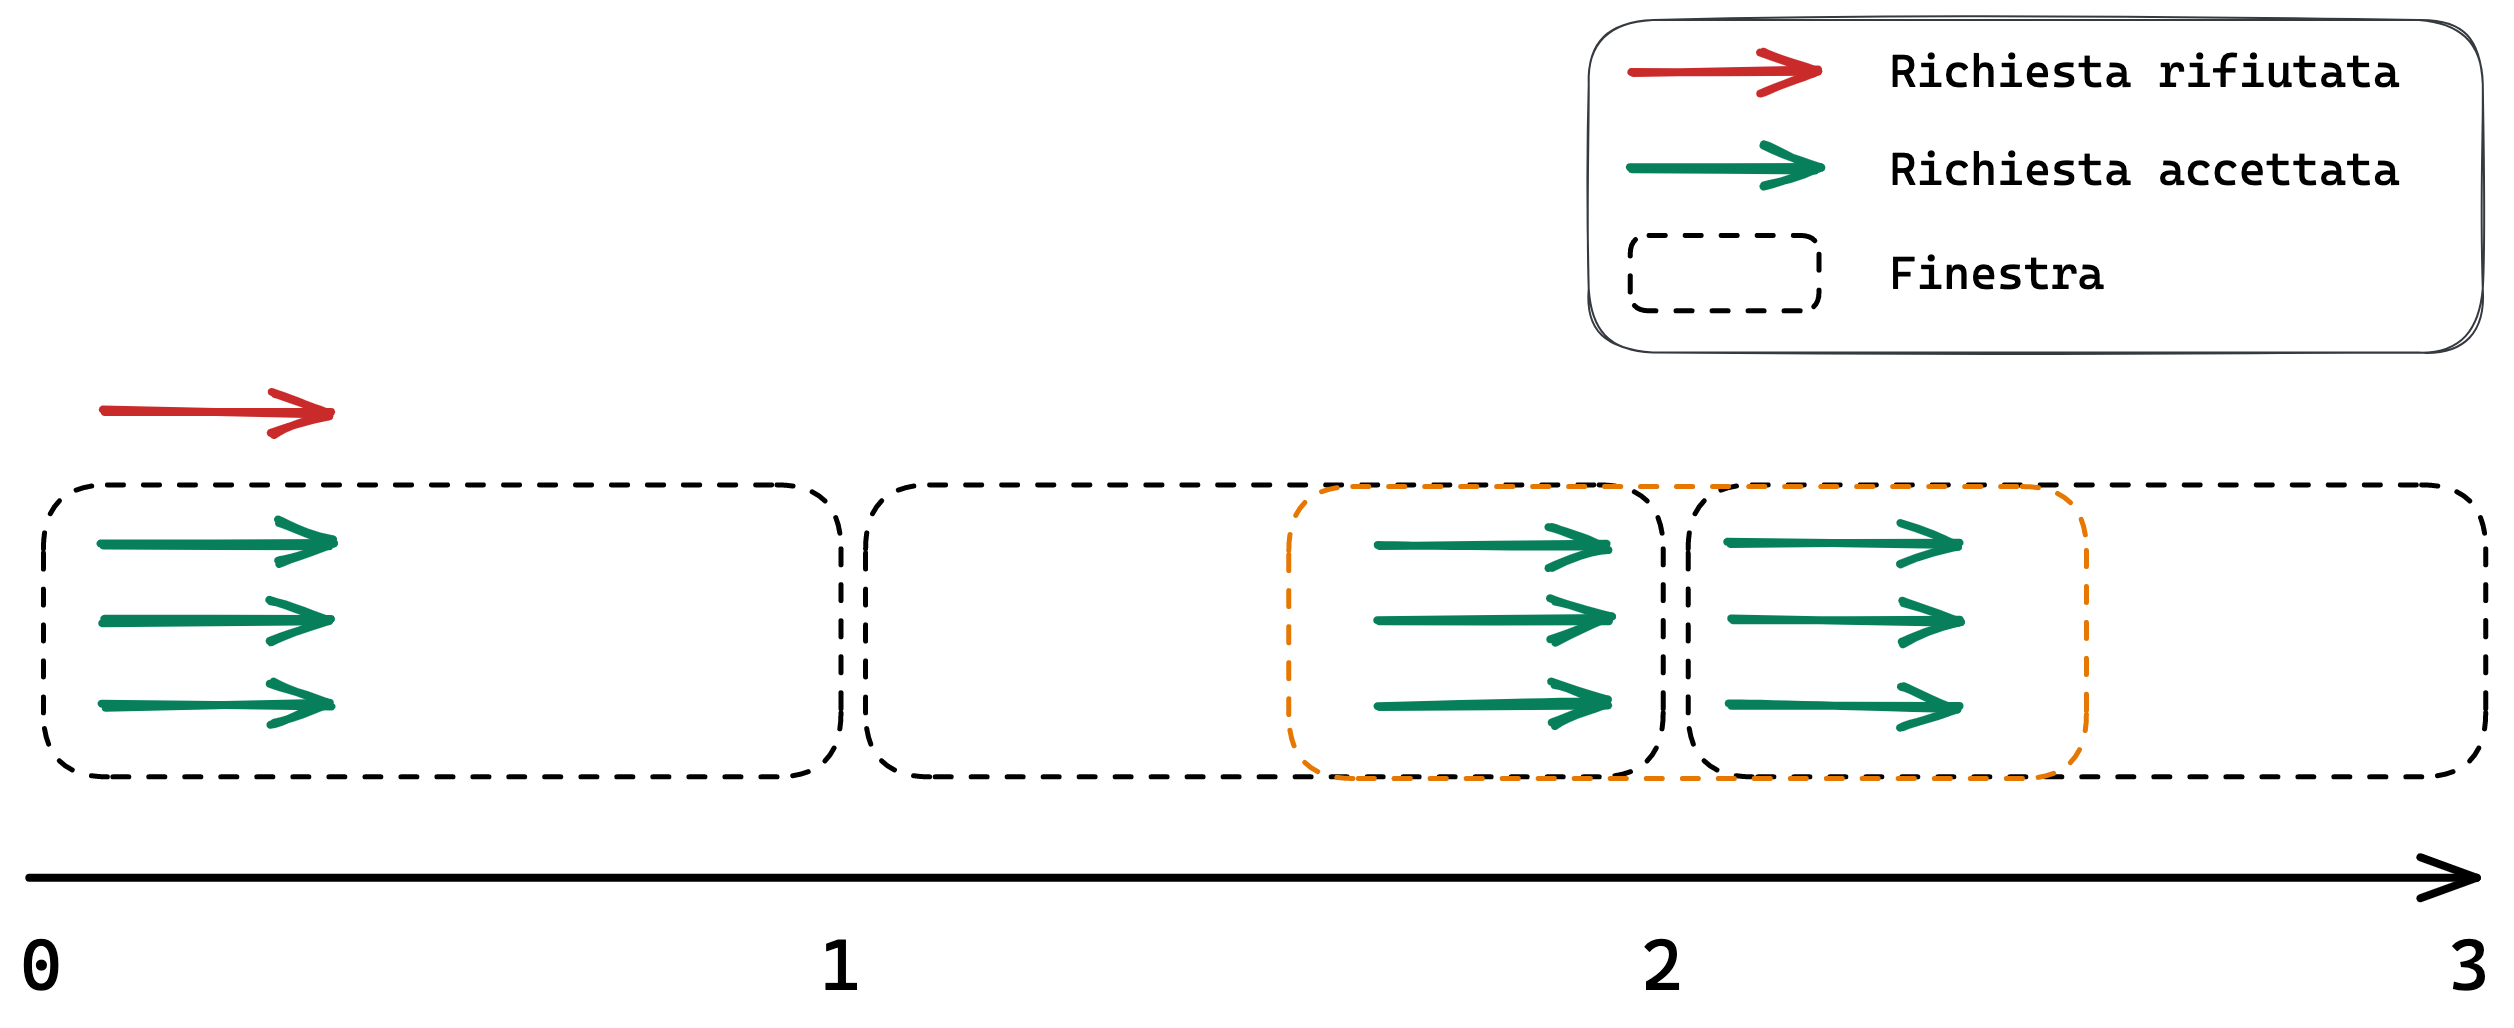
\includegraphics[width=13cm]{./chapters/1.state-of-art/images/1.fixed_window.png}
        \label{fig:fixed-window}
        \captionsetup{justification=centering}
        \caption{Strategia di rate-limiting: Fixed window}
    \end{figure}
    \item \textbf{Token bucket}: Il funzionamento del token bucket prevede che non tutte le richieste di un servizio vengano mappate
    1:1 con la richiesta di risorse, poiché alcune richieste potrebbero richiedere più risorse di altre. Per questo motivo,
    viene mantenuto un contatore di risorse, che viene scalato per ogni richiesta, del numero di token necessari per portare
    a termine il lavoro. Il contatore ha una frequenza di riempimento, ovvero a ogni unità di tempo viene reimpostato al suo
    valore massimo. Quando un utente o un'applicazione invia una richiesta al sistema, il sistema verifica se ci sono
    abbastanza token disponibili per soddisfare la richiesta. Se non ci sono abbastanza token, la richiesta viene respinta.
    In questo modo, le richieste vengono accettate solo se c'è abbastanza capacità per soddisfarle.
    \begin{figure}[h]
        \centering
        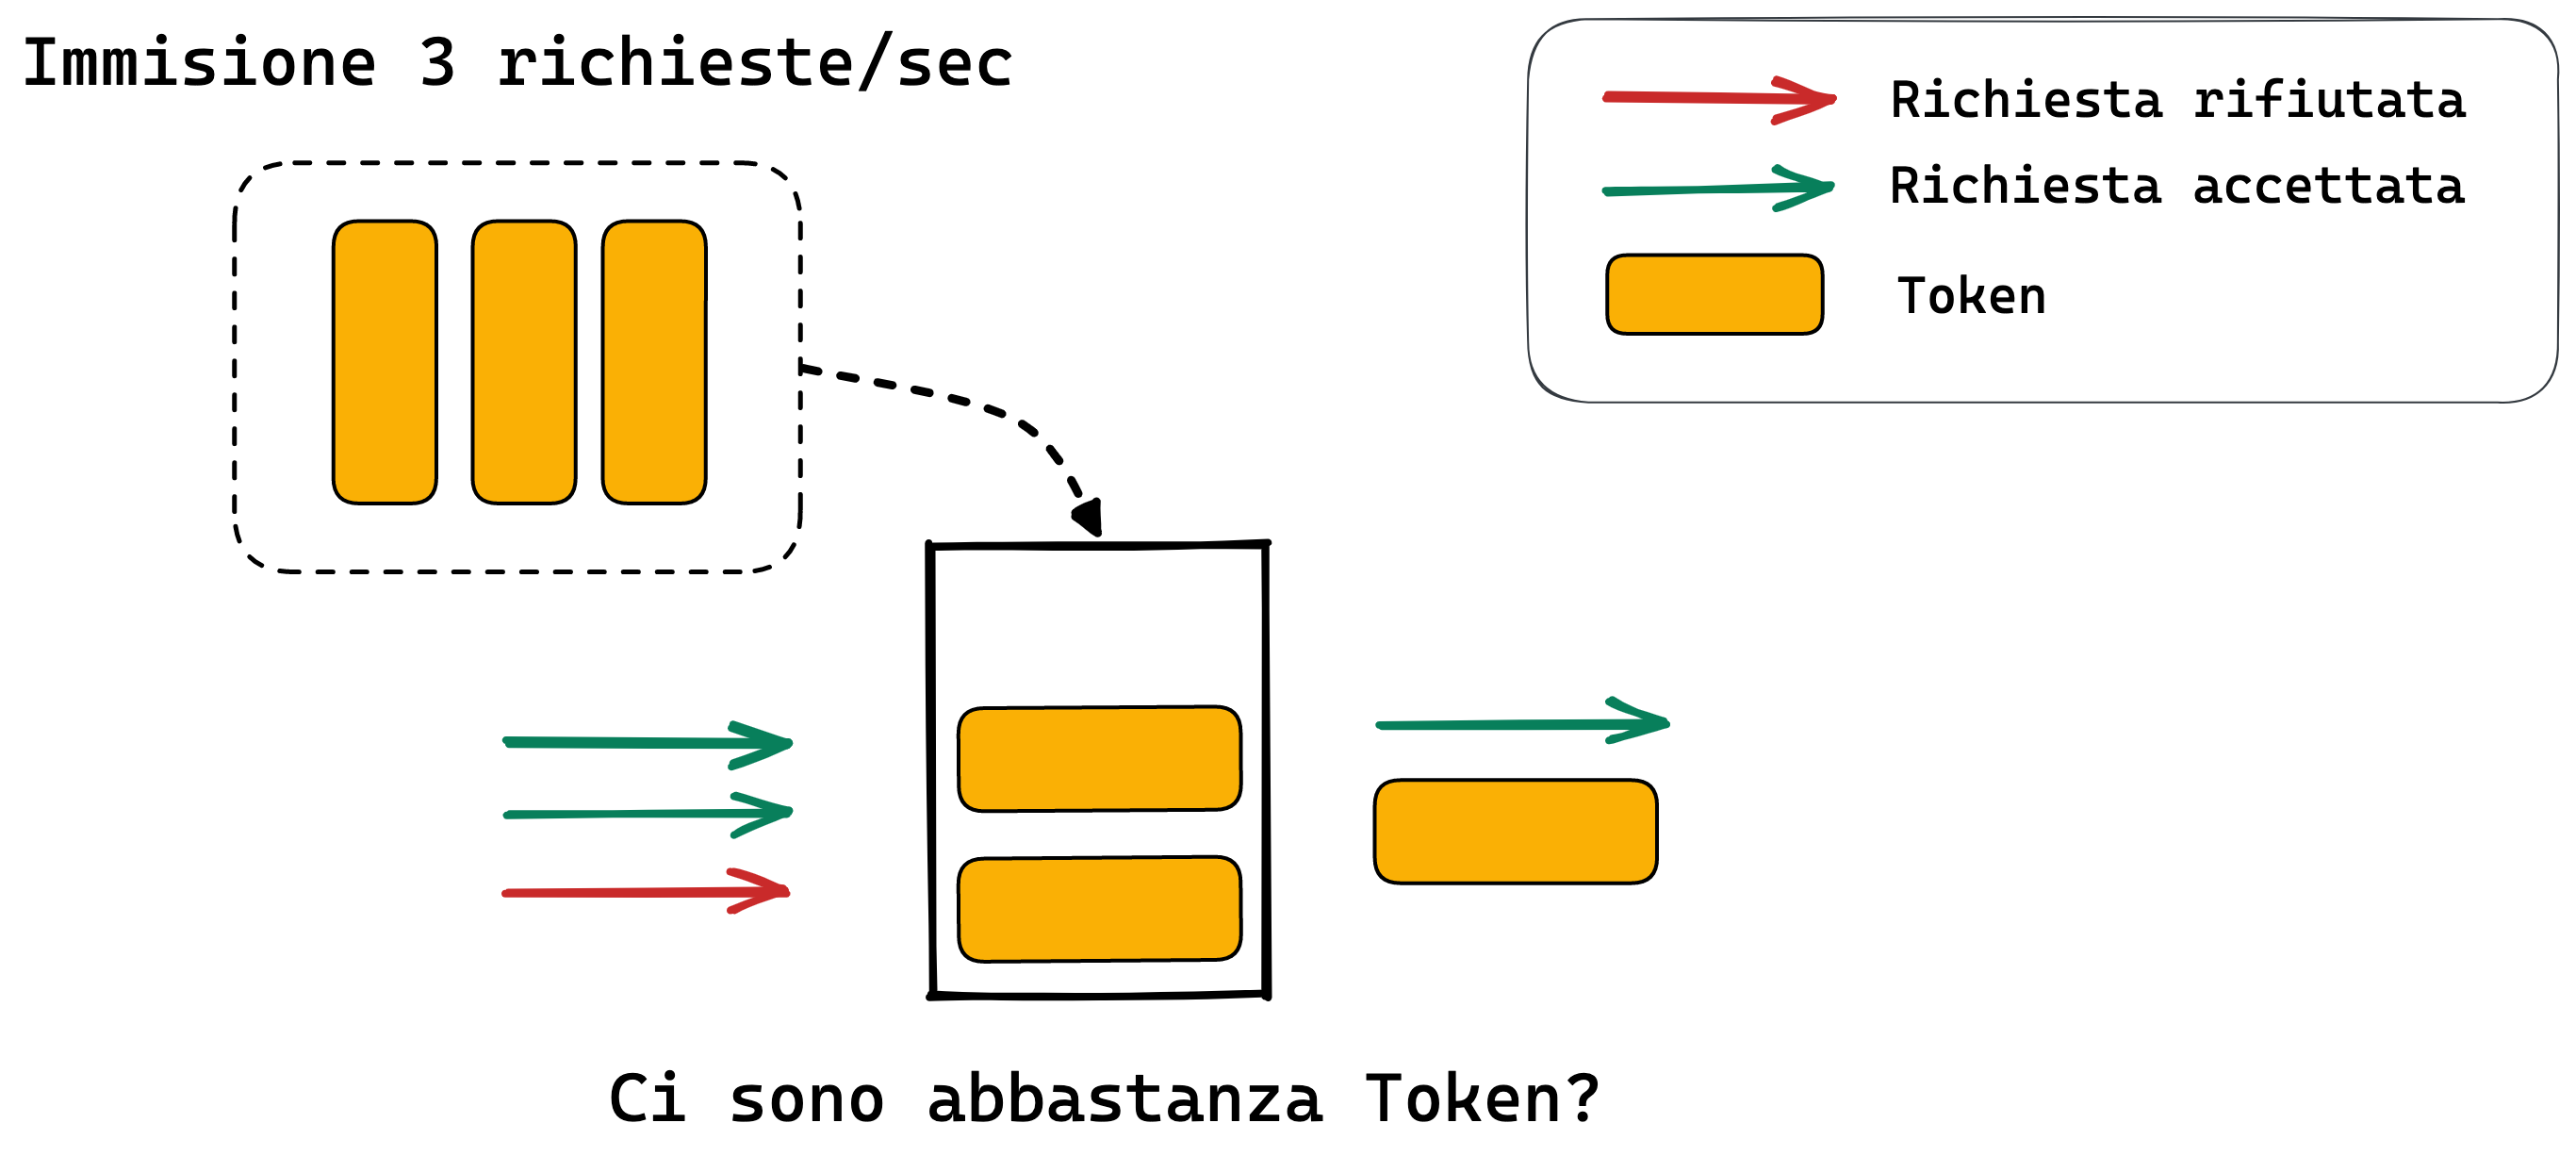
\includegraphics[width=13cm]{./chapters/1.state-of-art/images/2.token_bucket.png}
        \label{fig:token-bucket}
        \captionsetup{justification=centering}
        \caption{Strategia di rate-limiting: Token bucket}
    \end{figure}
    \item \textbf{Leaky bucket}: L'idea di base è simile a quella del Token bucket ma invece di rispondere al numero di richieste
    liberando i token necessari fino a esaurimento, il tasso di elaborazione delle richieste viene regolato in modo
    uniforme. Questo significa che quando un pacchetto di dati arriva al sistema, se il secchio è già pieno, il pacchetto
    viene scartato. Nel mentre ad ogni unità di tempo viene elaborata una quantità di richieste corrispondente alla velocità
    di uscita del sistema. In questo modo, il flusso di dati in uscita non supera mai una certa soglia.
    \begin{figure}[h]
        \centering
        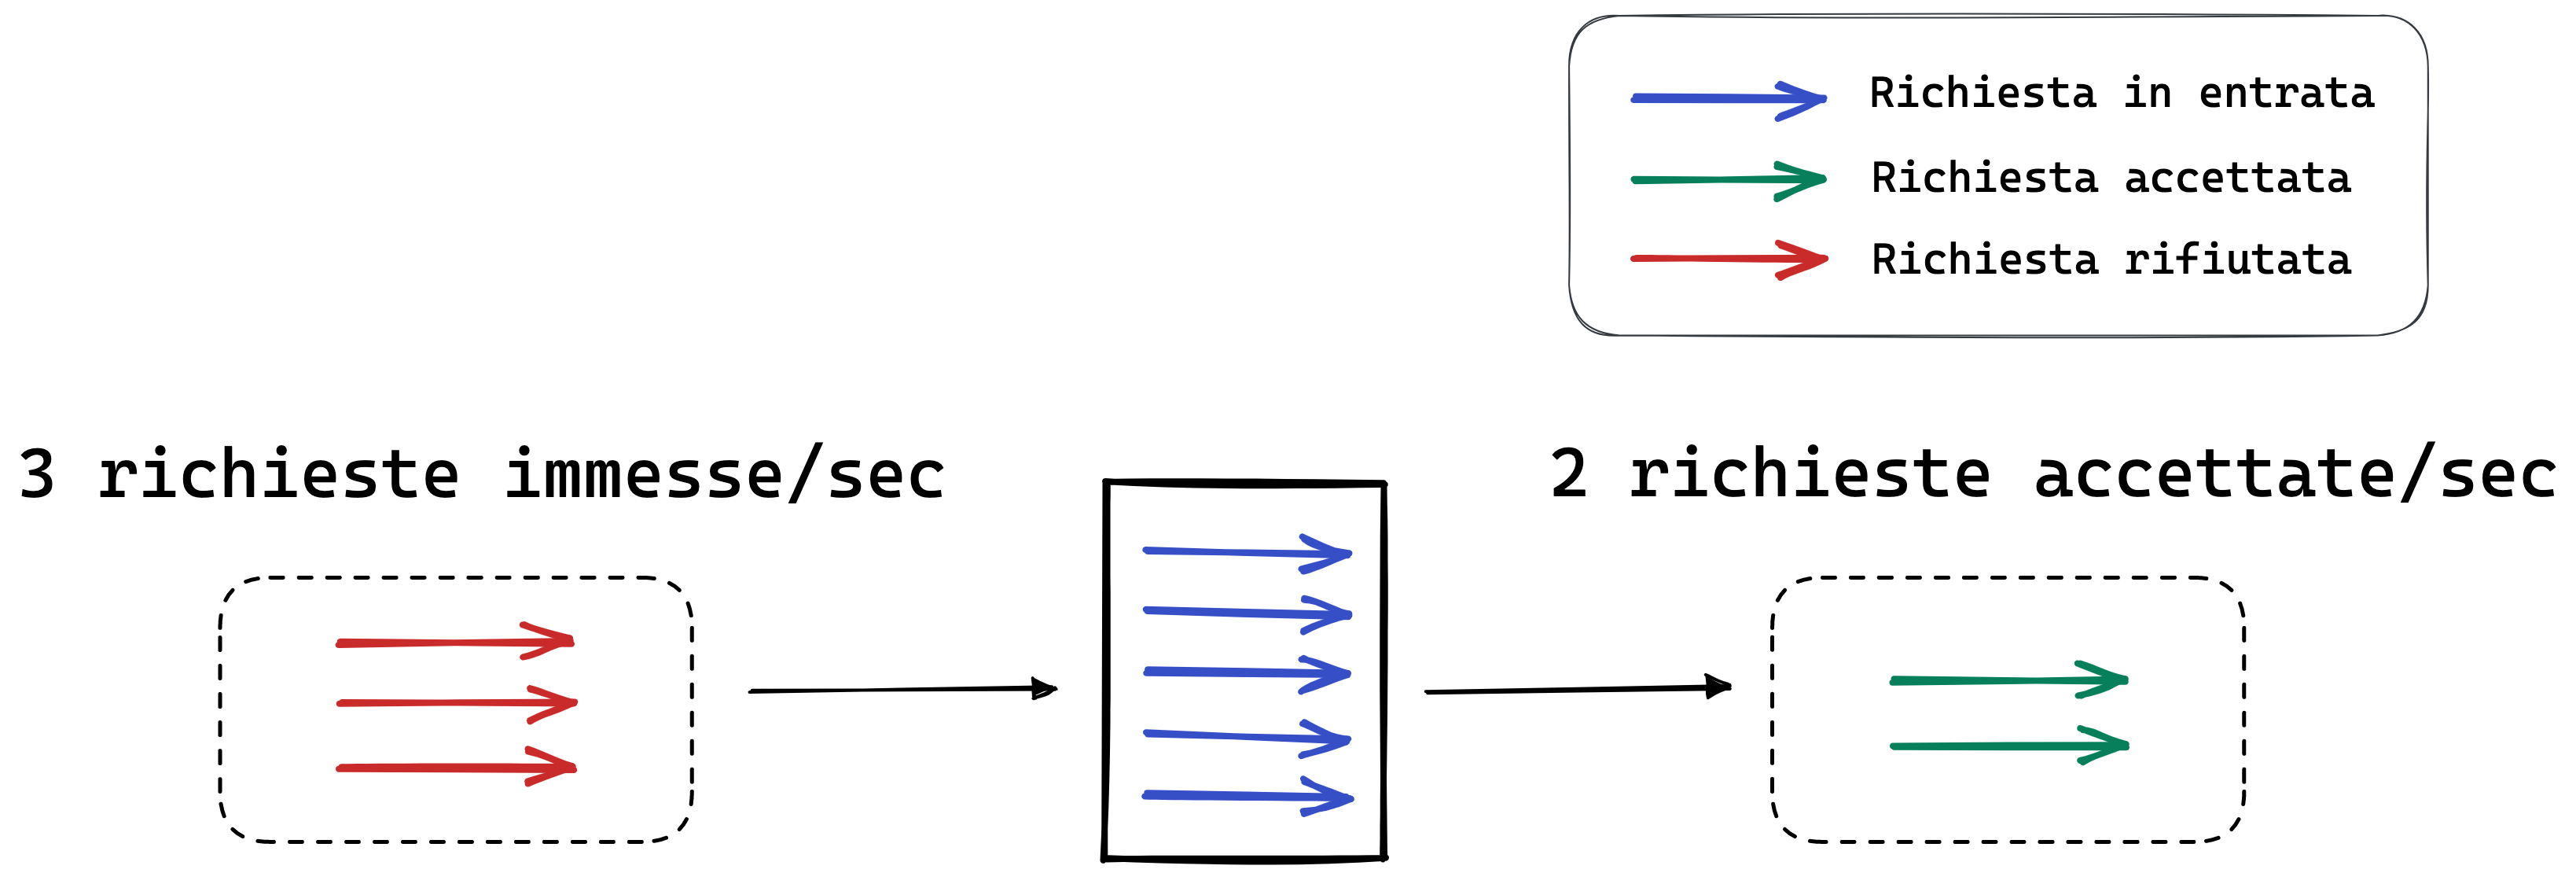
\includegraphics[width=13cm]{./chapters/1.state-of-art/images/3.leaky_bucket.png}
        \label{fig:laky-bucket}
        \captionsetup{justification=centering}
        \caption{Strategia di rate-limiting: Leaky bucket}
    \end{figure}
    \item \textbf{Sliding window}: La strategia di sliding window adotta un approccio simile alla Fixed Window, ma con una differenza
    fondamentale: esamina il tasso di richieste effettuate in un periodo di tempo continuo piuttosto che in intervalli
    fissi. Ad esempio, se il limite di richieste è fissato a 100 al minuto, la strategia prevede di controllare il numero di
    richieste effettuate nell'ultimo minuto e, nel caso superi il limite, rifiutare la richiesta. Questo approccio evita il
    potenziale sovraccarico del sistema alla fine di una finestra con un tempo prefissato, ma richiede la gestione di una
    finestra scorrevole, aumentando la complessità di implementazione.
    \begin{figure}[h]
        \centering
        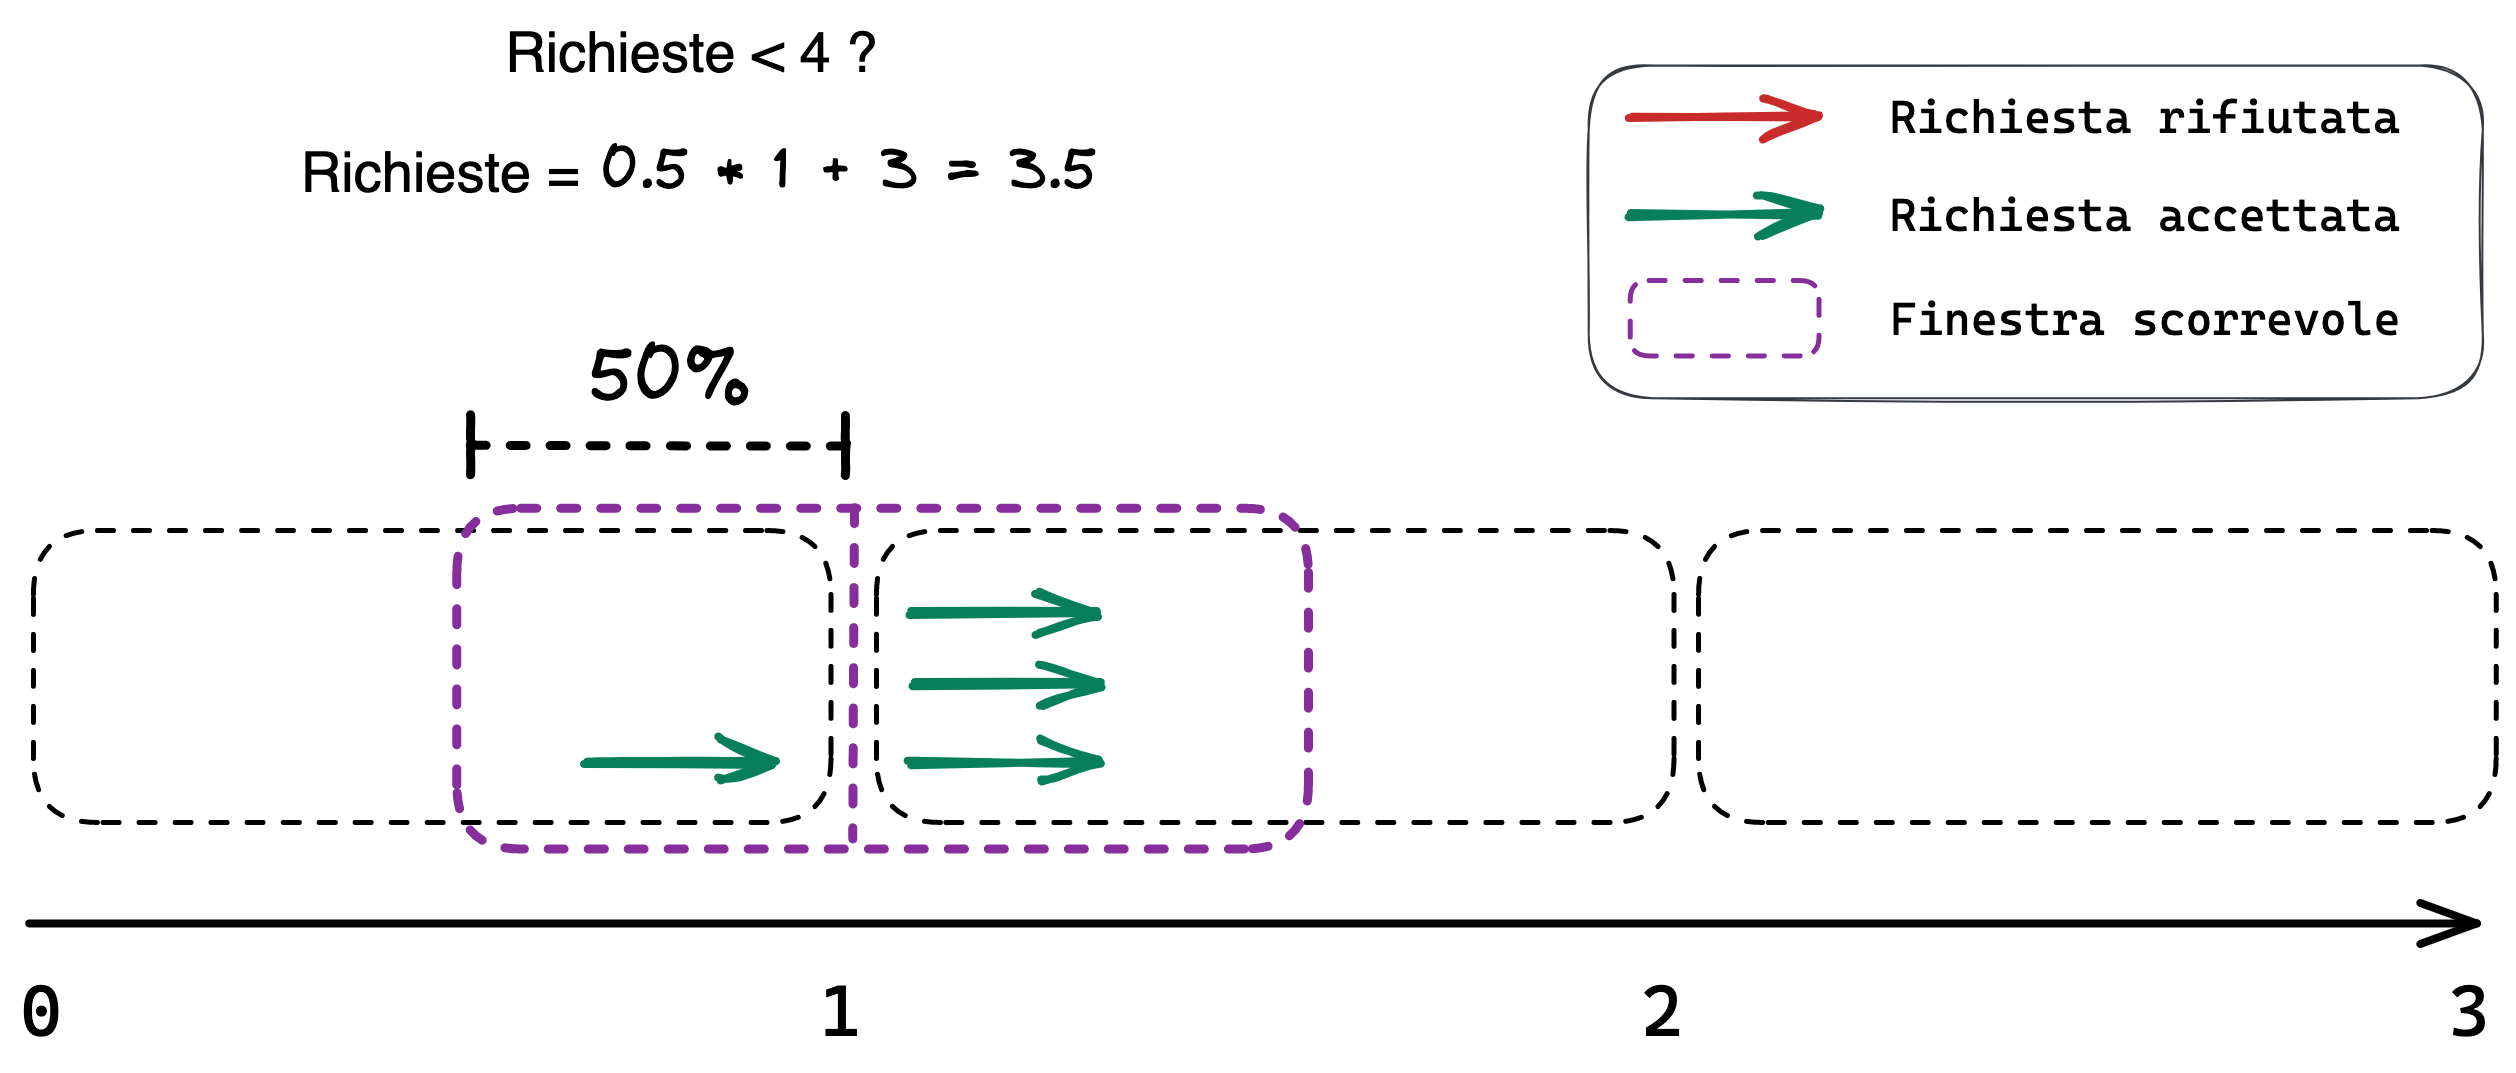
\includegraphics[width=13cm]{./chapters/1.state-of-art/images/4.sliding_window.png}
        \label{fig:sliding-window}
        \captionsetup{justification=centering}
        \caption{Strategia di rate-limiting: Sliding window}
    \end{figure}
\end{itemize}

Vale la pena notare che pur essendo un metodo ampiamente utilizzato il rate-limiting da solo potrebbe risultare
insufficiente per garantire un livello di sicurezza adeguato contro gli attacchi DoS, pertanto, è necessario adottare
contromisure di diversa natura al fine di garantire una protezione completa.
\clearpage
\section{zk-SNARK}

L'acronimo zk-SNARK rappresenta l'espressione completa "Zero-Knowled Succinct Non-Interactive Argument of Knowledge".
Questa tecnologia è stata formalizzata per la prima volta in un articolo scientifico pubblicato nel 2014 intitolato
"Succinct non-interactive zero knowledge for a von Neumann architecture"\cite{10.5555/2671225.2671275}. Da allora, sono state apportate diverse migliorie alla tecnologia
e sono emerse numerose applicazioni in svariati settori. Le prime applicazioni significative di zk-SNARK sono state
implementate nel contesto della Blockchain, che rimane il settore dove la tecnologia è più conosciuta e applicata, per
fare alcuni esempi Etherium\footnote{\url{https://ethereum.org}} una delle Blockchain più accreditate  ha iniziato ad implementare la tecnologia nella sua
rete dal 2016, e il suo fondatore Vitalik Buterin ha scritto in un articolo sull’argomento: “Perhaps the most powerful
cryptographic technology to come out of the last decade is general-purpose succinct zero knowledge proofs, usually
called zk-SNARKs” \cite{how-zk-snarks-are-possible} (Forse la tecnologia crittografica più potente emersa nell'ultimo decennio è quella delle prove
succinte a conoscenza zero di uso generale, solitamente chiamate zk-SNARK.).

Zk-SNARK, come suggerisce il nome, rappresenta una tecnologia fondata sul protocollo crittografico zero-knowledge proof,
il quale consente a una parte (il dimostratore) di dimostrare a un'altra (il verificatore) la veridicità di
un'affermazione senza rivelare nessuna informazione ulteriore. Inoltre questo processo di dimostrazione, viene
effettuato in modo da ottenere una prova, in cui sia la dimensione della prova, che il tempo necessario per verificarla
crescono molto più lentamente rispetto al calcolo da verificare e senza la necessità di interazione bidirezionale tra le
due parti coinvolte.

Di seguito esamineremo meglio le singole parti che compongono la tecnologia zk-SNARK, analizzando i suoi componenti
chiave per ottenerne una panoramica completa.

\textbf{Notare}: Nei prossimi paragrafi lavoreremo nel dominio algebrico dei campi finiti.

\subsection{Zero-Knowledge}

Come accennato precedentemente, Zero-Knowledge proof è un protocollo crittografico in cui una parte dimostra di
conoscere una determinata informazione a un'altra parte, senza rivelare alcuna informazione aggiuntiva su di essa. Per
esempio, se Peggy vuole dimostrare a Victor di conoscere la password del suo account, senza rivelargli la password stessa,
può utilizzare un protocollo di tipo Zero-Knowledge. In questo modo, Peggy può dimostrare a Victor di sapere quale è la
password corretta senza rivelarla, proteggendo così la sua privacy e la sicurezza del suo account.

Formalmente le prove di tipo Zero-Knowledge non sono dimostrazioni di carattere matematico, ma probabilistiche, il che
significa che c'è sempre una probabilità che un dimostratore disonesto riesca a dimostrare la veridicità di
un'affermazione a un verificatore onesto. Esistono tuttavia tecniche per ridurre questa probabilità a valori piccoli a
piacere.

Il primo articolo che definisce il costrutto è “The Knowledge Complexity of Interactive Proof-Systems"\cite{10.1145/22145.22178} pubblicato nel
1985, dove  gli autori introducono il concetto di “Zero-Knowledge proof” come un tipo di "interactive proof
systems" \cite{interactive_proof_system} (un modello computazionale che simula lo scabio di
messagi tra due individui) in cui il verificatore non apprende nulla oltre alla verità dell'affermazione che viene
dimostrata.

Per poter ottenere un sistema Zero-Knowledge proof per una particolare affermazione abbiamo bisogno che la prova
generata soddisfi le seguenti prorpietà :
\begin{itemize}
    \item \textbf{Completezza}: Se l'affermazione da dimostrare è vera, allora un verificatore onesto (cioè che segue correttamente le
    regole del protocollo) verrà convinto della veridicità da un dimostratore onesto.
    \item \textbf{Correttezza}: Se l'affermazione è falsa, nessun dimostatore disonesto può convincere un verificatore onesto che essa è vera, se non con una piccola
    probabilità.
    \item \textbf{Zero-knowledge}: se l'affermazione è vera, nessun verificatore apprende altro se non il fatto che
    l'affermazione è vera.
\end{itemize}
Le tre proprietà appena viste descrivono un sistema Zero-Knowledge proof da un punto di vista formale ma per avere una visione più
intutiva del protocollo è utile vedere il funzionamento del protocollo attraverso un esempio. L’esempio in questione è tratto
da un famoso articolo di Jean-Jacques Quisquater "How to Explain Zero-Knowledge Protocols to Your Children” \cite{10.1007/0-387-34805-0_60}  ne
estrapolerò solo le parti esenziali alla tratazione, ma ne consiglio la lettura.

L’esempio riguarda una caverna a forma di anello, nella quale è posta a metà del percoso una porta che impedisce il
passaggio, a meno di non conoscere una parola segreta. Supponiamo l'esistenza di due parti, Peggy - che
conosce il segreto della porta e agirà da dimostratrice - e Victor - che invece non conosce il segreto e sarà il
verificatore. Peggy vuole dimostrare a Victor di sapere come superare la barriera senza però rivelare il segreto. Per
fare ciò, Peggy propone a Victor di seguire una strategia: dapprima stabiliscono un nome per identificare i due percorsi
(ad esempio, A e B), poi Victor rimane fuori dalla caverna mentre Peggy sceglie uno dei due percorsi. 
\begin{figure}[H]
    \centering
    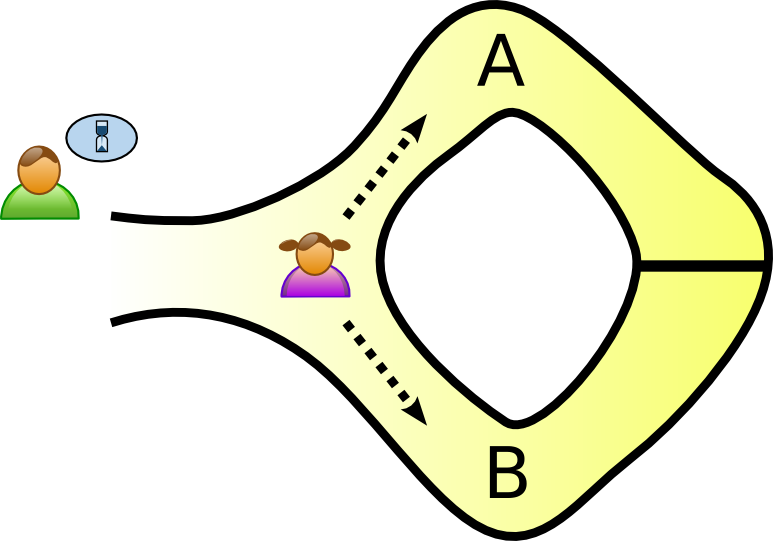
\includegraphics[width=5cm]{./chapters/1.state-of-art/images/5.1.alibaba_cave.png}
    \label{fig:alibaba-cave1}
    \captionsetup{justification=centering}
    \caption{Disegno della caverna}
\end{figure}
Dopo qualche minuto, Victor entra nella caverna e chiama ad alta voce il nome di uno dei due percorsi, a quel punto Peggy dovrà
uscire dal percorso chiamato da Victor. 
\begin{figure}
    \centering
    \begin{subfigure}{.5\textwidth}
        \centering
        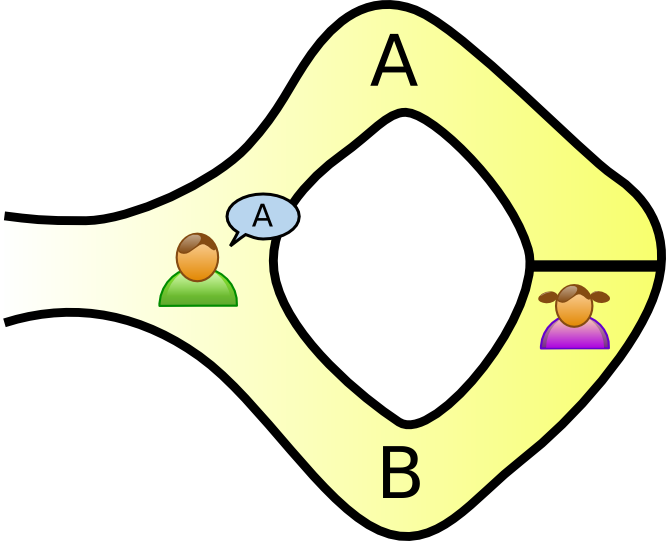
\includegraphics[width=4cm]{./chapters/1.state-of-art/images/5.2.alibaba_cave.png}
        \label{fig:alibaba-cave2}
        \captionsetup{justification=centering}
    \end{subfigure}%
    \begin{subfigure}{.5\textwidth}
        \centering
        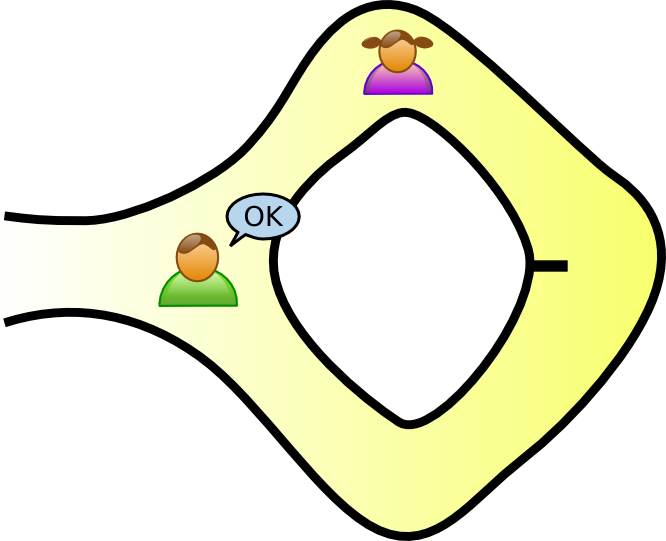
\includegraphics[width=4cm]{./chapters/1.state-of-art/images/5.3.alibaba_cave.png}
        \label{fig:alibaba-cave3}
        \captionsetup{justification=centering}
    \end{subfigure}
    \caption{Interzione tra Peggy e Victor}
    \label{fig:alibaba-cave2_3}
\end{figure}
Victor accetta la proposta, ma con una condizione: il processo dovrà essereBob
ripetuto più volte. Dopo diversi tentativi, Victor si convince che Peggy conosca effettivamente il segreto per superare
la barriera. Possiamo calcolare questa probabilità utilizzando la distribuzione binomiale, dove la probabilità di
successo p è del 50\% e il numero totale di prove n è 10. La probabilità di indovinare correttamente tutte le 10 scelte
di Victor è data dalla seguente formula: \(P = p^n = 0,5^{10} = 0,0009765625\)

L'esempio proposto è molto efficace nel far comprendere come sia possibile dimostrare il possesso o la conoscenza di un
informazione senza rivelarla. Nell’articolo citato inoltre si prevendono diversi scenari in cui una o entrambe le parti
potrebbero essere disoneste. Per gestire tali situazioni, è possibile applicare una procedura denominata "trusted
setup", che verrà approfondita nelle sezioni relativa alle prove non interattive \hyperref[sec:non-interactive]{[Non-Interactive]}.

\subsection{Succinct}
Una dimostrazione di tipo succinct che potremmo tradurre con la parola concisa, è una prova in cui sia la dimensione
della prova che il tempo necessario per verificarla crescono molto più lentamente rispetto alla computazione da
verificare. Ad esempio se Peggy volesse provare a Victor di possedere un array composto da un milione di elementi, dove
ogni elemento è uguale all’indice dell’array più uno.

\begin{equation}
a = [1,2,3,...,1000000]
\end{equation}

Una prova di tipo succinct, così come definita, non può essere realizzata attraverso un processo di controllo "uno per
uno" degli elementi dell'array. Questo perché, se così fosse, si otterrebbe un processo che richiederebbe tanto tempo e
spazio di memoria quanto il calcolo effettuato per generare l'array. Una possibile miglioria rispetto al calcolo puntuale
potrebbe essere quella di campionare l'array in un punto casuale e controllare se l'elemento selezionato rispetta la
regola. \\
Dopo un singolo campionamento, il grado di fiducia di Victor rispetto ad Peggy sarebbe di soli 0,0001\%, ovvero un
milionesimo. Se in uno qualsiasi dei campionamenti effettuati Victor dovesse prelevare un numero non congruo, la
dimostrazione verrebbe invalidata completamente senza bisogno di ulteriori controlli. È possibile aumentare il grado di
fiducia del verificatore eseguendo più controlli, ma anche in questo caso, le prove generate da dimostratori disonesti
in cui uno o pochi elementi sono errati all'interno dell'intera prova richiederebbero un numero eccessivo di passaggi
per raggiungere un grado di fiducia accettabile, rendendo cosi questo secondo approccio fragile e non attuabile.

\begin{figure}[H]
    \centering
    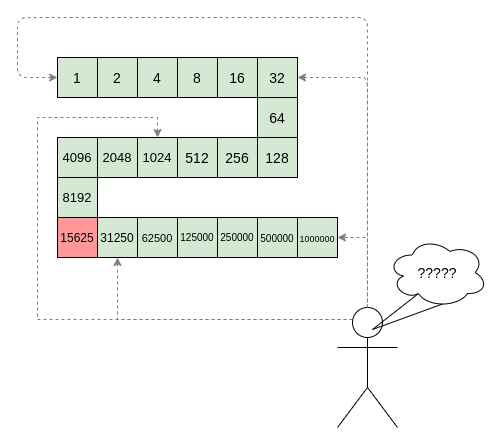
\includegraphics[width=9cm]{./chapters/1.state-of-art/images/6.hope_evaluation.png}
    \label{fig:hope-evaluation}
    \captionsetup{justification=centering}
    \caption{Disegno esempio di valutazione a tentativi fallita}
\end{figure}

\subsubsection{Polinomi}

Per trovare una soluzione al problema, è necessario fare riferimento ai polinomi, in particolare alla tecnica
crittografica nota come "polynomial commitments". Questa tecnica ci consente di generare delle funzioni hash per i
polinomi, chiamate "polynomial commitment", sulle quali è ancora possibile effettuare operazioni algebriche. Ciò
significa che possiamo eseguire operazioni sui polinomi senza conoscerli, attraverso i commitment. L'utilizzo di questa
tecnica ci fornisce notevoli vantaggi durante la fase di verifica, Infatti la possibilità di verificare le informazioni
del dimostratore senza dover operare un controllo puntuale è possibile grazie a una proprietà dei polinomi descritta dal
lemma di Schwartz-Zippel; un risultato importante in teoria della complessità
computazionale e della teoria degli algoritmi che stabilisce una condizione sufficiente per determinare se un polinomio
multivariato non nullo ha radici in un campo finito.

Per comprendere come questo strumento possa esserci utile, partiamo da un equivalenza intuitiva: ipotizzando di essere
in possesso di due polinomi $f(x_1,...,x_n)$ e $g(x_1,...,x_n)$, chiedersi se $f \equiv g$ è
equivalente a chiedersi se 

\begin{equation}
p(x_1,...x_n) = f(x_1,...x_n)-g(x_1,...x_n) \equiv 0
\end{equation}

L'intuizione su cui possiamo basarci per capire l’utilità del lemma per i nostri fini, è che Victor (il verificatore) abbia il polynomial
commitment  $g(x_1,...,x_n)$ del polinomio corretto $f(x_1,...,x_n)$ e voglia verificare che Peggy (il dimostratore) lo
conosca. \clearpage
Sotto quete ipotesi possiamo immaginare un semplice protocollo di esempio dove:
\begin{enumerate}
    \item  Victor sceglie un punto qualsiasi $s$ e valuta il suo polynomial commitment in $s$, e ottiene $g(s_1,...,s_n)$.
    \item  Victor invia $s$ a Peggy che provvederà a valutare il suo polinomio in $s$, e ottiene $f(s_1,...,s_n)$.
    \item  Peggy invia il risultato della sua valutazione a Victor che la confronta con il suo valore, se i
    valori sono uguali Victor si convince che nel punto $s$ Peggy consce il corretto polinomio.
\end{enumerate}

In questa fase ci potremmo chiedere quale beneficio abbiamo ottenuto passando dalla formulazione dell'array in cui
venivano fatti campionamenti casuali, alla formulazione dei polinomi in cui vengono fatte valutazioni del polinomio in
variabili casuali. Il beneficio è dovuto al lemma di Schwartz-Zippel, che permette di dimostrare che:

Prendendo un polinomio $p(x_1,...,x_n$) di grado $d > 1$ con coefficienti in un campo finto $\mathbb{K}$, prendendo 
$S \subset \mathbb{K}$ e $r_1,...,r_n \in S$ scelti in modo arbitrario, allora se $p(x_1,...,x_n$) non è il polinomio nullo
abbiamo che $p(r_1,...,r_n) = 0$ con probabilità $\le \ d/|S|$

Nell'immagine sottostante si può osservare che prendendo un polinomio qualunque nel campo finito $\mathbb{K}$, la
probabilità che il polinomio valutato in un punto casuale sia uguale a 0 differisce di poco se calcolata con la
definizione classica di probabilità o con il lemma di Schwartz-Zippel, tuttavia il calcolo attraverso la seconda formula è molto più immediato.
\begin{figure}[H]
    \centering
    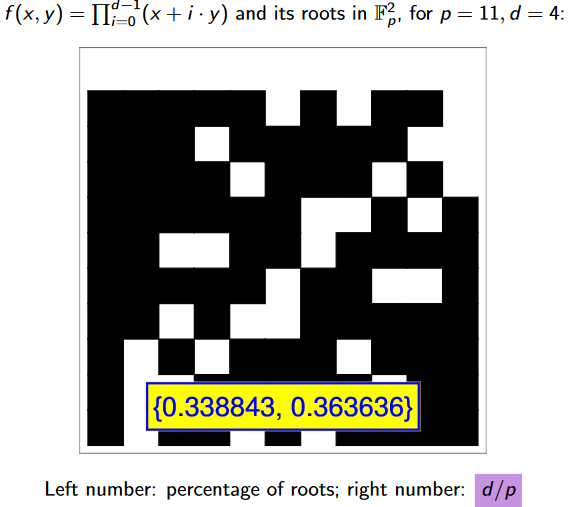
\includegraphics[width=10cm]{./chapters/1.state-of-art/images/7.schwartz_zippel_lemma.png}
    \label{fig:schwartz-zippel-lemma}
    \captionsetup{justification=centering}
    \caption{Esempio applicazione del lemma di Schwartz-Zippel, tratta da \cite{23-schwartz-zippel}}
\end{figure}
\clearpage

La conseguenza del lemma è che la probabilità di trovare una radice del polinomio in un gruppo di valori appartenenti al
campo è inferiore o uguale al rapporto tra il grado del polinomio e la cardinalità del gruppo di elementi selezionati,
operazione molto più veloce da calcolare di un controllo puntuale. Inoltre se decidessimo di ripetere il processo di
selezione degli $r_1,...,r_n \in S$ un numero k di volte otterremo che la probabilità che $p(r^k_1,...,r^k_n) = 0$
sarebbe obbligatoriamente $\le \ (d/|S|)^k$  e per valori di $S$ abbastanza grandi il il rapporto tende molto velocemente
a 0. Intuitivamente il lemma ci dimostra che se un'equazione che coinvolge alcuni polinomi è vera in una coordinata
selezionata arbitrariamente, allora è quasi certamente vera per i polinomio nel suo insieme.

\subsubsection{Come calcolare i polinomi}

Una volta compreso il vantaggio nell'affrontare il problema mediante l'utilizzo di polinomi, possiamo
procedere alla descrizione del processo che ci permette di ottenere tali polinomi.

\begin{figure}[H]
    \centering
    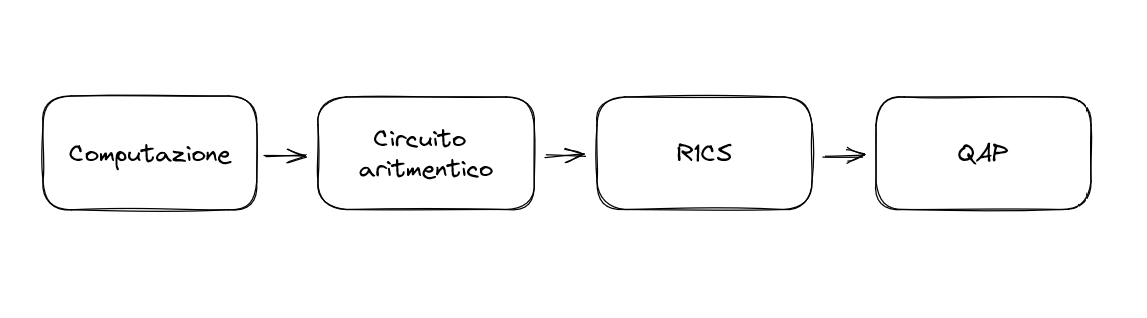
\includegraphics[width=14cm]{./chapters/1.state-of-art/images/8.comp_qap.png}
    \label{fig:comp-qap}
    \captionsetup{justification=centering}
    \caption{Passi da seguire per ottenere un QAP}
\end{figure}

Per illustrare in dettaglio i passaggi che conducono dalla computazione alla rappresentazione polinomiale desiderata,
ovvero la QAP (Quadratic Arithmetic Programs), utilizzeremo un compilatore scritto in Rust\footnote{\url{https://www.rust-lang.org}} chiamato circom\footnote{\url{https://docs.circom.io/}}

\begin{enumerate}
    \item  La prima fase, ovvero il passaggio dalla computazione al circuito algebrico, può essere un processo non immediato,
    soprattutto quando si trattano computazioni articolate. A titolo di esempio, consideriamo la computazione $2*x^2=18$ con
    l'ovvia soluzione da dimostrare $x=3$. Per ottenere un circuito algebrico a partire da questa computazione, si può
    procedere come segue:\clearpage
        
    \begin{figure}[H]
        \centering
        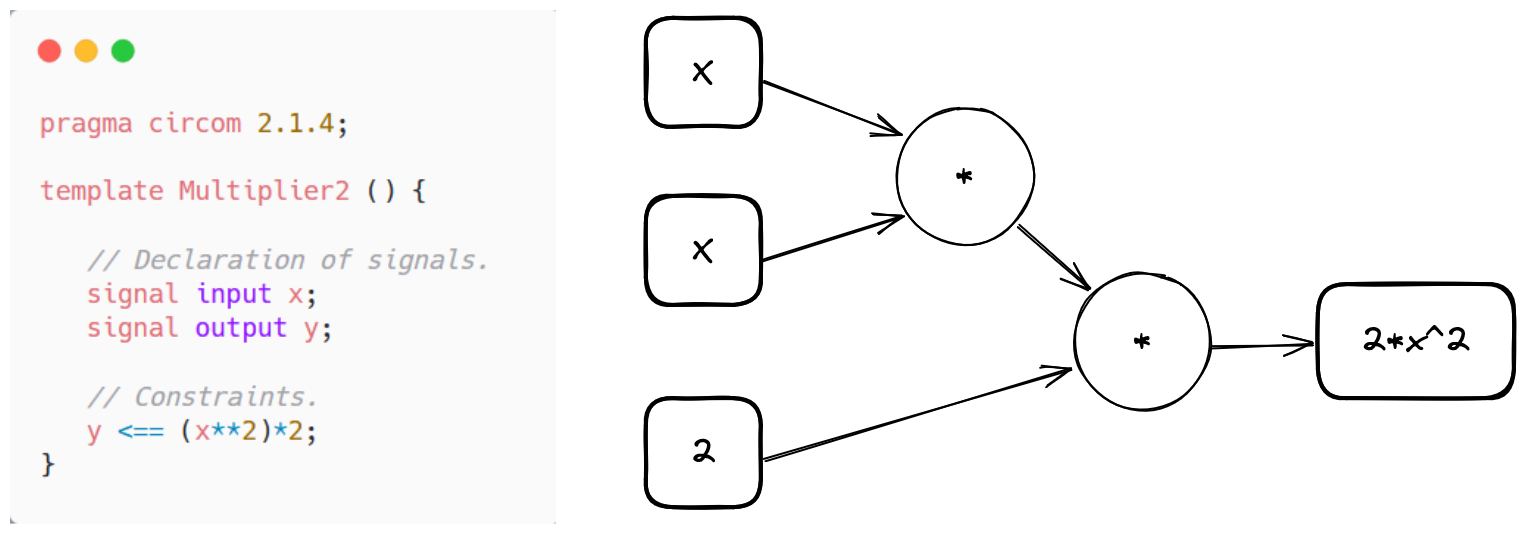
\includegraphics[width=13cm]{./chapters/1.state-of-art/images/9.comp_circ.png}
        \label{fig:comp-circ}
        \captionsetup{justification=centering}
        \caption{Codice esemplificativo per la creazione di un circuito algebrico}
    \end{figure}

    \item  Ora per proseguire dobbiamo trasformare il nostro circuito aritmetico in un formato chiamato R1CS. R1CS è un
    formato in cui ogni vincolo (gate del circuito) viene espresso tramite in una terna di vettori (a,b,c) e sul quale viene
    calcolato un vettore chiamo $s$ che rappresenta la soluzione del sistema di vincoli R1CS. Il vettore $s$ è
    costruito nel seguente modo:
    $$
    s \cdot a * s \cdot  b - s \cdot  c = 0
    $$
    
    dove con il simbolo $\cdot$  si rappresenta il prodotto scalare. Continuando con il nostro esempio dal circuito
    precedente possiamo calcolare le terne di vettori $(a,b,c)$ per i due gate
    \begin{gather*}
        A =
        \begin{bmatrix}
        0 & 1 & 0 & 0 \\
        0 & 0 & 0 & 1 \
        \end{bmatrix}
        \qquad
        B =
        \begin{bmatrix}
        0 & 1 & 0 & 0 \\
        2 & 0 & 0 & 0 \
        \end{bmatrix}
        \qquad
        C =
        \begin{bmatrix}
        0 & 0 & 0 & 1 \\
        0 & 0 & 1 & 0 \
        \end{bmatrix}
    \end{gather*}
        
    Possiamo osservare che per ognuno dei due gate del circuito, sono stati creati una terna di vettori $(a,b,c)$ di
    dimensione 4, la dimensione dei vettori è dovuta al numero di variabili del circuito. \\
    Per quanto riguarda il vettore $s$, esso viene calcolato a partire dal vettore delle variabili del circuito,
    inserendo al posto di ogni variabile il valore assunto durante la valutazione del circuito. In questo modo, il
    vettore $s$ rappresenta la soluzione del sistema R1CS.

    \begin{gather*}
        \text{Vettore variabili} =
        \begin{bmatrix}
            one, & x, & out, & sym_1 \\
        \end{bmatrix}
        \\
        \\
        \text{Vettore} \ s =
        \begin{bmatrix}
        1 & 3 & 18 & 9 \\
        \end{bmatrix}
    \end{gather*}

    Possaimo vedere che $sym_1$ è una variabile creata per spezzare il calcolo di $2*x^2$ in due diversi vincoli più
    semplici questa procedura viene chiamata "Flattening" (appiattimento), mentre $one$ è una variabile di sistema
    utilizzata per effettuare operazioni algebriche come la moltiplicazione o la somma per gli elementi del campo. Per
    verificare che il vettore $s$ sia effettivamente una soluzione del sistema di vincoli R1CS, è possibile calcolare la
    formula precedente per ogni gate del circuito.

    \begin{figure}[H]
        \centering
        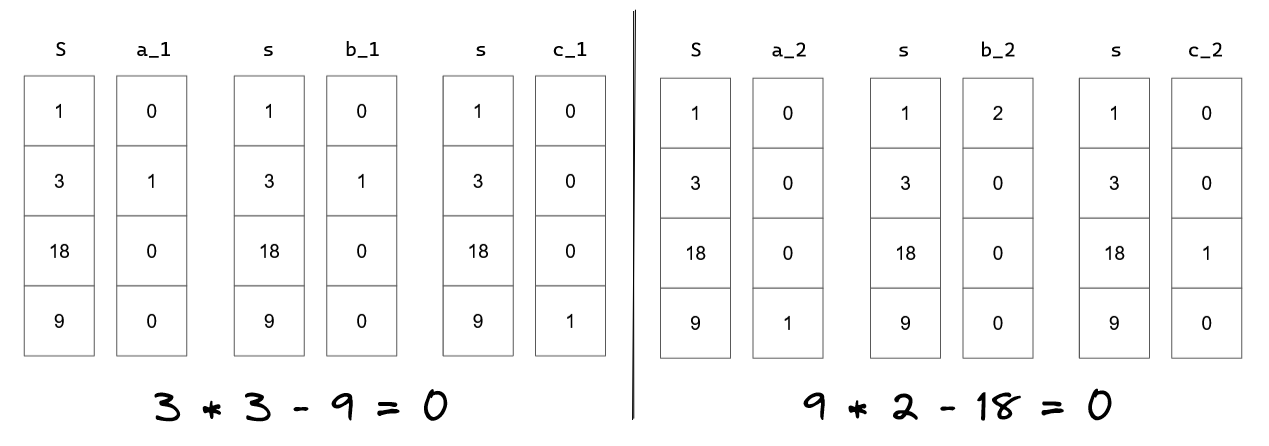
\includegraphics[width=15cm]{./chapters/1.state-of-art/images/10.check_r1cs.png}
        \label{fig:check-r1cs}
        \captionsetup{justification=centering}
        \caption{Contrllo dei vincoli R1CS}
    \end{figure}

    Visto che il risultato dell'operazione è 0 possiamo dire che $s$ è una soluzione del sistema R1CS, e quindi che il
    nostro valore $x=3$ che compone il vettore soluzione è corretto. Al pari del calcolo puntuale delgli esempi
    precedenti questa operazione di verifica per circuiti con molti gate non può essere percorribile.

    \item  Il processo di trasformazione dal formato R1CS al formato QAP è il più complesso e richiede l'utilizzo di una
    tecnioca chiamata interpolazione di Lagrange. L'idea principale è quella di costruire dei polinomi tali che se
    valutati nelle coordinate relative ai vincoli, restituiscano i valori dei vettori corrispondenti. Il processo per
    ottenere i polinomi si basa su una procedura iterativa su i vettori delle matrici $A,B$ e $C$. 
    Applicando il processo al nostro esempio otteniamo i seguenti polinomi:
    \begin{gather*}
        \text{Ap} =
        \begin{bmatrix}
        0x^2+0x \\
        -1x^2+2x \\
        0x^2+0x \\
        1x^2-1x \
        \end{bmatrix}
        \qquad
        \text{Bp} =
        \begin{bmatrix}
        2x^2-2x \\
        -1x^2+2x \\
        0x^2+0x \\
        0x^2+0x \
        \end{bmatrix}
        \qquad
        \text{Cp} =
        \begin{bmatrix}
        0x^2+0x \\
        0x^2+0x \\
        1x^2-1x \\
        -1x^2+2x \
        \end{bmatrix}
    \end{gather*}    
    Questi polinomi sono costruiti in modo tale che valutandoli in x = 1 (coordinata del primo vincolo) otteniamo i valori corrispondenti ai vettori del
    primo vincolo
    \begin{gather*}
        \text{Ap} =
        \begin{bmatrix}
        0&\
        1&\
        0&\
        0\
        \end{bmatrix}
        \qquad
        \text{Bp} =
        \begin{bmatrix}
        0&\
        1&\
        0&\
        0\
        \end{bmatrix}
        \qquad
        \text{Cp} =
        \begin{bmatrix}
        0&\
        0&\
        0&\
        1\
        \end{bmatrix}
    \end{gather*}
    grazie a questa formato ora se volessimo verificando i vincoli tramite la formula precedente avremmo
    
    $$
    A(x)*B(x)-C(x)=P(x)
    $$
    
    dove $P(x)$ non è obbligatoriamente il polinomio nullo. Tuttavia Se la dimostrazione è corretta $P(x)$ deve avere delle
    radici in tutti le coordinate corrispondenti ai vincoli. Per verificarlo non abbiamo bisogno di controllare tutti i
    vincoli perché lavorando con i polinomi possiamo sfruttare il lemma di Schwartz-Zippel per valutare la condizione
    molto più velocemente.
\end{enumerate}
    
\subsubsection{Valutazioni sul protocollo}
Fino ad ora abbiamo descritto un processo che ci consente di trasformare i nostri vincoli numerici in polinomi,
permettendoci di calcolare con grande velocità e un elevato grado di certezza la validità dei vincoli imposti. Tuttavia,
il protocollo spiegato in precedenza presenta due falle:

\begin{enumerate}
    \item \textbf{Arbitrarietà}: Nel secondo passaggio del protocollo, Victor condivide con Peggy un punto $s$, che è stato scelto
    casualemten per valutare il polinomio. Tuttavia, passando $s$ in chiaro ad Peggy ci si espone al rischio che Peggy
    costruisca un polinomio ad hoc, che soddisfi i vincoli solo nel punto specifico scelto, permettendole così di convincere
    Victor di pur non conoscendo il polinomio. Ciò violerebbe il principio di correttezza dei protocolli Zero-Knowledge proof.
    \item \textbf{Verificabilità}: la capacità di Peggy di valutare correttamente il polinomio in $s$ non garantisce che essa abbia
    utilizzato effettivamente il polinomio $p$ per restituire il risultato a Victor, In altre parole, non è garantito che Peggy
    abbia utilizzato il polinomio descritto dal polynomial commitment per raggiungere il risultato atteso.
\end{enumerate}

Per affrontare questi due problemi, vengono utilizzate altre tecniche matematiche, denominate Homomorphic Encryption (HH) per
risolvere il primo problema e Knowledge of Coefficient (KC) per risolvere il secondo. In questa sede, si accennerà
brevemente a come è possibile ottenere un Homomorphic Encryption in grado di soddisfare la proprietà di correttezza,
mentre la trattazione del KC non verrà approfondita. È possibile trovare una introduzione ad entrambe le tecniche
in questa serie di articoli \cite{explaining_sanrks}

\subsubsection{Homomorphic Encryption}

L'idea alla base dell'Homomorphic Encryption è quella di costruire un'operazione simile all'operazione di hashing con la
proprietà di poter applicare delle operazioni aritmetiche ai valori criptati senza decifrarli, ovvero ottenere una
funzione $E(x)$ che soddisfi tali proprietà :
\begin{enumerate}
    \item \textbf{Difficoltà di inversione}: Dato un  $E(x)$ sia complesso risalire a $x$
    \item \textbf{Resistenza alle collisioni}: Se $x \ne y \Rightarrow E(x) \ne E(y)$
    \item \textbf{Preserva operazioni aritmetiche}: Se si conoscono E(x) ed E(y), si può generare
    delle espressioni aritmetiche in x e y. Per esempio, si può calcolare E(x+y) da E(x) ed E(y)
\end{enumerate}
\clearpage

\subsection{Non-Interactive}
\label{sec:non-interactive}

Tutti i protocolli Zero-Knowledge proof esaminati fino ad ora erano di tipo interattivo. Questo significa che per
generare e verificare la prova, le due parti coinvolte, ovvero il verificatore e il dimostratore, devono interagire in
modo bidirezionale. Ad esempio, nel caso della "grotta di Alibaba", Victor, il verificatore, indicava il passaggio da
intraprendere e Peggy, il dimostratore, che “rispondeva” uscendo dalla giusta direzione. Mentre nel caso dei
polinomi, il verificatore forniva le coordinate del punto in cui valutare il polinomio e il dimostratore rispondeva con
la valutazione corretta. In alcune situazioni tuttavia, può risultare vantaggioso utilizzare le cosiddette NIZKP, ovvero
le Non-Interactive Zero-Knowledge proof, in cui il dimostratore trasmette al verificatore una prova contenente tutte le
informazioni necessarie per la verifica, senza richiedere ulteriori interazioni tra le parti. 

Questa metodologia presenta numerosi vantaggi sia in termini di prestazioni, poiché consente di costruire le prove più
velocemente senza dover attendere la risposta e il tempo di comunicazione, sia in termini di sicurezza, in quanto
l'assenza di uno scambio di messaggi elimina il rischio di intercettazioni da parte di individui malintenzionati.
Inoltre, l'utilizzo di prove NIZKP potrebbe risultare obbligato in quei contesti applicativi in cui la comunicazione in
tempo reale non è possibile. L'adozione di questo tipo di prove comporta però un aumento della complessità, poiché,
essendo privi di interazione, tutto il lavoro di generazione e preparazione alla verifica viene svolto dal dimostratore
e affinché il dimostratore non sia arbitrariamente libero di agire, generando prove scorrette, è necessario vincolarlo
al rispetto delle regole. 

A tal fine, si utilizza una tecnica nota come "trusted set-up" che consente di generare una Common Reference String
(CRS), ovvero un dato pubblico conosciuto sia dal dimostratore che dal verificatore usato per aggiungere casualità
all’interno della generazione della prova. Sempre riferendoci ai due esempi precedenti, la CRS ottenuta tramite un
trusted set-up consentirebbe di rendere le scelte di Victor nella caverna il più casuali possibile, impedendo ad Peggy
di individuare dei pattern o a entrambi di collaborare per ingannare un terzo osservatore e nel caso dei polinomi,
invece, consentirebbe di rendere aleatoria la scelta del punto in cui valutare il polinomio. 

La procedura di costruzione della CRS rappresenta un passaggio critico per la robustezza del protocollo e dipende
fortemente dal tipo di cerimonia di trusted set-up scelta.

\subsubsection{Modello di affidabilità}

Una cerimonia di trusted set-up è una procedura che viene eseguita una sola volta per generare un CRS che poi potrà
essere utilizzata ogni volta che viene eseguito il protocollo. Il termine "trusted" deriva dal fatto che una o più
persone devono partecipare alla cerimonia in modo “fidato” contribuendo alla creazione della CRS con dei segreti anche
chiamati “toxic waste” che non appena inseriti nella procedura dovranno essere eliminati. \clearpage

Una volta completata l'elaborazione e dopo aver eliminato i segreti, il risultato dell'elaborazione (la CRS) diventa
irreversibile e non può essere riprodotta volontariamente, il che garantisce la sicurezza del protocollo.
\begin{figure}[H]
    \centering
    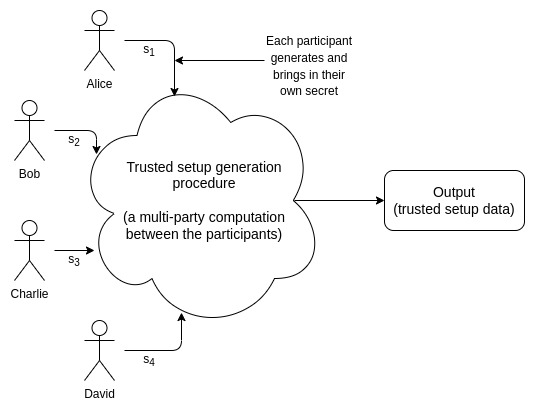
\includegraphics[width=10cm]{./chapters/1.state-of-art/images/11.trusted_setups.png}
    \label{fig:trusted_setups}
    \captionsetup{justification=centering}
    \caption{immagine generica di una cerimonia di trusted set-up. tratta da \cite{how-do-trusted-setups-work}}
\end{figure}

Se le parti coinvolte non si comportano in modo leale e conservano o pubblicano i loro segreti, la validità della
cerimonia dipenderà dal modello di affidabilità utilizzato dall'algoritmo di trusted set-up. Infatti poiché i protocolli
operano in diversi domini applicativi, non tutti utilizzano lo stesso modello di affidabilità. 

Una trattazione completa dei vari modelli di affidabilità esula dai miei scopi, tuttavia, riducendo la classificazione a due sole proprietà
degli algoritmi, è possibile descrivere brevemente alcune tipologie utili per la trattazione successiva. 

Le due proprietà su cui si basa la classificazione sono il numero di parti fidate che partecipano alla cerimonia e il numero di
parti che devono comportarsi “lealmente” per garantire la segretezza della CRS.

In base a queste proprietà, si possono individuare tre gruppi di interesse (non sono gli unici):
\begin{itemize}
    \item \textbf{1 - 1}: Questo modello è simile a quello utilizzato nei servizi centralizzati, in cui ci si affida a un singolo
    individuo fidato per la gestione dei dati. 
    \item \textbf{N/2 - 1}: La maggior parte delle blockchain utilizza questo modello, in
    cui il processo viene considerato valido se la maggioranza dei partecipanti rimane onesta.
    \item \textbf{1 - N}: In questo modello, è sufficiente che almeno una delle parti rimanga onesta durante la
    cerimonia per garantire la segretezza della CRS.
\end{itemize}

\begin{figure}[H]
    \centering
    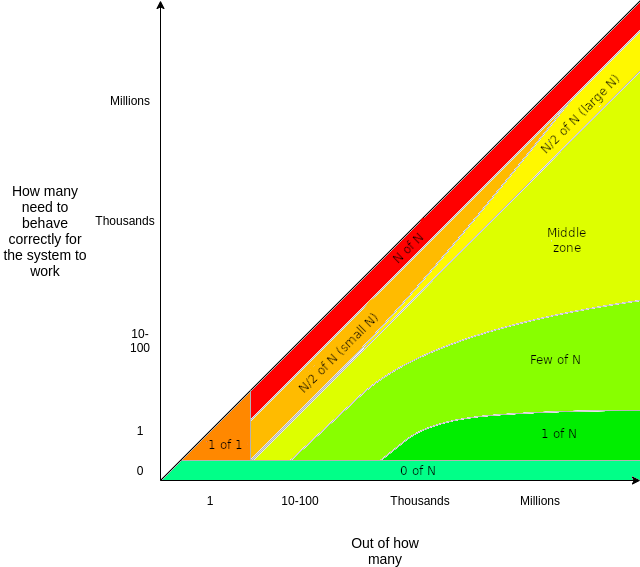
\includegraphics[width=10cm]{./chapters/1.state-of-art/images/12.trusted_models.png}
    \label{fig:trusted_models}
    \captionsetup{justification=centering}
    \caption{immagine modelli di di affidabilità, tratta da \cite{trusted-models}}
\end{figure}

\subsubsection{MPC (multi-party computation)}
La tecnologia MPC (multi-party computation), anche se non è stata ancora esplicitamente menzionata, è alla base dei
trusted set-up. Infatti per generare una CRS sicura e non riproducibile, è necessario coinvolgere molte parti e
garantire che nessuno possa ricavare informazioni sui segreti dei partecipanti o sulla CRS stessa. Per questo motivo la
procedura non si limita a una semplice combinazione dei segreti, ma può essere vista come una "black box" che applica
elaborazioni ai segreti in input e restituisce la CRS in output.

Ogni algoritmo di MPC deve soddisfare due proprietà fondamentali:

\begin{enumerate}
    \item Nel caso in cui uno o più partecipanti disonesti decidano di rivelare il loro segreto, il protocollo MPC deve
    impedire loro di obbligare i partecipanti onesti a rivelare le loro informazioni riservate o influenzare il risultato
    finale.
    \item Nessuno dei partecipanti deve essere in grado di dedurre i segreti degli altri partecipanti dagli elaborati
    del protocollo. In altre parole, il calcolo effettuato dall'algoritmo non deve fornire alcun indizio sui segreti che
    hanno portato al risultato.
\end{enumerate}

\subsubsection{Groth16}
Groth16 è un protocollo Zero-knowledge proof proposto da Jens Groth nell’articolo “On the Size of Pairing-based
Non-interactive Arguments” \cite{10.1007/978-3-662-49896-5_11} pubblicato nel 2016, questo protocollo è diventato molto
diffuso grazie alla sua grande efficienza dal punto di vista computazionale, che permette di creare zk-SNARK
estremamente performanti sia in termini di tempo che di memoria. Tale tecnologia è alla base di progetti come Z-cash\footnote{\url{https://z.cash/}}.

Il trusted set-up su cui si basa Groth16 richiede due fasi distinte:
\begin{enumerate}
    \item Nella prima fase si applica una procedura di trusted set-up chiamata “power of tau” che consiste in una algoritmo MPC
    basato sul modello di affidabilità 1-N che utilizzando le curve ellitice permette di generare una CRS. Il processo viene
    chiamato powers of tau o Pot perchè duarnte le sue fasi vengono usate le potenze di un numero tao generalmente il 2
    assime ai contributi dei partecipanti per generare punti casuali e ottener una CRS. il numero N di partecipati per una
    cerimonia di tipo power of tau puo essere dell'ordine del migliaio di partecipanti rendendo cosi la cerimonia molto
    sicura, in quanto basta che almento uno di essi mantenga il segreto per far si che la CRS rimanga valdia. Questo
    procedimento deve essere svolto una volta sola e deve essere combinato con il processo della fase successiva.
    \begin{figure}[H]
        \centering
        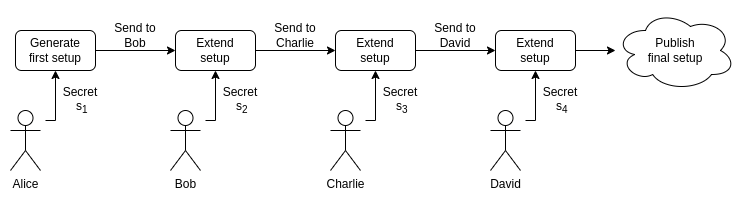
\includegraphics[width=13cm]{./chapters/1.state-of-art/images/13.power_of_tao.png}
        \label{fig:powers_of_tao}
        \captionsetup{justification=centering}
        \caption{immagine generica di una di power of tau. tratta da \cite{how-do-trusted-setups-work}}
    \end{figure}
    \item Nella seconda fase invece viene elaborato un trusted set-up dipendente dalla computazione che si vuole provare (o
    meglio dipendete dal circuito). Quindi questa fase deve essere riprodotta dal dimostratore ogni volta che la
    dimostrazione cambia. Non entrerò nei dettagli implementativi, ma in questa fase viene utilizzata l' euristica di Fiat-Shamir
    , che permette di scegliere il punto in cui valutare il polinomio, che descrive la computazione, senza che il
    dimostratore possa interferire. Il punto viene scelto sulla base dei calcoli fatti per ottenere il polinomio stesso. È
    intuitivo comprendere che se il dimostratore volesse falsificare la prova, non potrebbe farlo perché per scegliere
    arbitrariamente un polinomio pere soddisfare un determinato vincolo, dovrebbe conoscere il valore di $s$ ma essendo
    $s$ derivato dal polinomio stesso questo non è possibile.
\end{enumerate}

Indubbiamente il fatto che la robustezze della tecnologia zk-SNARK sia subordinata a una procedura cosi elaborata è uno
svantaggio, infatti esistono, protocolli di Zero-knowledge proof che non necessitano di una fase di trust set-up
iniziale. Bulletproof e le STARK (Scalable Transparent Arguments of Knowledge), ad esempio, non richiedono alcuna
configurazione di questo tipo, ciò nonostante, le tecnologie  zk-SNARK basate su Groth16 risultano essere più performati in termini di
efficienza il che le rende molto più diffuse delle altre tecnologie.
\begin{figure}[H]
    \centering
    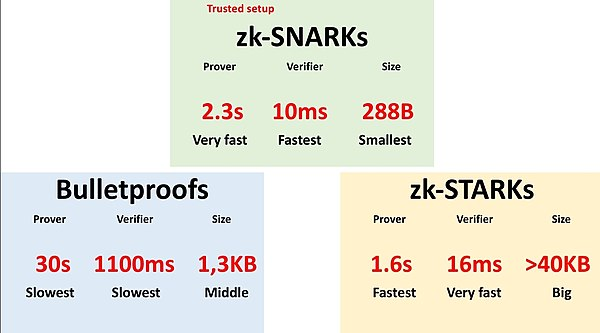
\includegraphics[width=13cm]{./chapters/1.state-of-art/images/14.diff_zk.png}
    \label{fig:different_zk}
    \captionsetup{justification=centering}
    \caption{immagine prestazioni di teconlogi NIZKP a confronto. tratta da \cite{non_interactive_zero_knowledge_proof}}
\end{figure}
\chapter{Analisi del protocollo RLN}
\chaptermark{Analisi del protocollo RLN}
\label{chap:rln-protocol}

Nel presente capitolo, tratteremo la discussione del protocollo RLN (Rate Limiting Nullifier), che consente la
costruzione di regole di rate-limiting anti DoS e spam in ambiente anonimo. La prima proposta del protocollo è stata
sviluppata da Barry WhiteHat, un ricercatore attivo nel campo della blockchain e delle applicazioni Zero Knowledge, nel
seguente post: "Semaphore RLN, rate limiting nullifier for spam prevention in anonymous p2p setting". Attualmente, RLN
fa parte di (PSE) Privacy \& Scaling Explorations, un team multidisciplinare sostenuto dalla Fondazione Ethereum, che
esplora nuove tecnologie Zero Knowledge e altre primitive crittografiche. Alcuni progetti di rilievo includono zk-kit,
Interep e Semaphore. RLN è ancora un protocollo poco conosciuto, e non esistono ancora grosse implementazioni al di
fuori del contesto di ricerca. Il progetto in stato più avanzato è relativo a un lavoro portato avanti da Vac che sta
lavorando sull'implementazione del protocollo all'interno di Waku v2, la seconda versione di un protocollo di
comunicazione peer-to-peer privacy-preserving in ambiente decentralizzato.

Il meccanismo RLN prima di tutto impone agli utenti di generare una chiave privata che sarà utlizzata per ricavare un identity commitment utilizzando la funzione hash Poseidon. In seguito per registrarsi, gli utenti devono fornire il loro identity commitment, che viene memorizzato in una foglia dell'albero di Merkle, il quale rappresenta la struttura dati dei membri del servizio. Per evitare attacchi di tipo Sybil il protocollo dà la possibilità di richiedere agli utenti in fase di registrazione anche una "stake" ovvero un informazione di valore appartenente all'untente che sia di difficiele riproducibilità. 

Per ogni interazione con l'applicazione, gli utenti devono generare una prova per dimostrare l'appatenenza all'albero di Merkle e devono rialscaire una prozione della loro chiave privata, dimostrando che si tratti effettivamente di una parte valida di essa. Durante questa procedura non vogliamo che nessuna informazione venga rilascaita oltre alla appartenenza e alal correttezza della porzione di chiave e per fare ciò sfruttiamo la tecnologia zk-SNARK

Per evitare lo spam, RLN implementa una regola anti-spam generale in cui gli utenti non possono effettuare più di X interazioni per epoca. Questo può essere applicato utilizzando lo schema di condivisione dei segreti di Shamir per dividere la chiave segreta in n parti, e se gli utenti effettuano più interazioni di quelle consentite per epoca, la loro chiave segreta può essere ricostruita.

Infine, il meccanismo RLN consente agli utenti di essere rimossi dall'albero di appartenenza da chiunque conosca la loro chiave segreta. Se si verifica un evento di spam, lo stake economico dello spammer può essere inviato al primo utente che segnala correttamente lo spammer fornendo la chiave segreta ricostruita dello spammer come prova.

Prima di esaminare in dettaglio lo sviluppo delle singole parti, analizzeremo gli strumenti utilizzati dal protocollo
per implementare le sue funzionalità.

\section{Strumenti}
\subsection{Alberi di Merkle}

Gli alberi di Merkle sono una particolare struttura ad albero che sfrutta le proprietà delle funzioni di hash al fine di
ottimizzare le operazioni di ricerca e identificazione delle modifiche all'interno della collezione. La struttura degli
alberi di Merkle è composta dalle foglie, che rappresentano i dati a cui è stata applicata una funzione di
hash e dai nodi, che sono ottenuti uno dopo l'altro applicando la funzione hash ai loro figli, fino a raggiungere
la radice. Negli alberi di Merkle la radice è una funzione hash che rappresenta univocamente la struttura. Per capire
meglio il concetto immaginiamo di avere un struttura ad albero binaria, e inseriamo all'interno della struttura gli
elementi 1,2,3,4 e 5 a cui applichiamo una funzione hash, a questo punto otterremo la seguente struttura:
\begin{figure}[H]
    \centering
    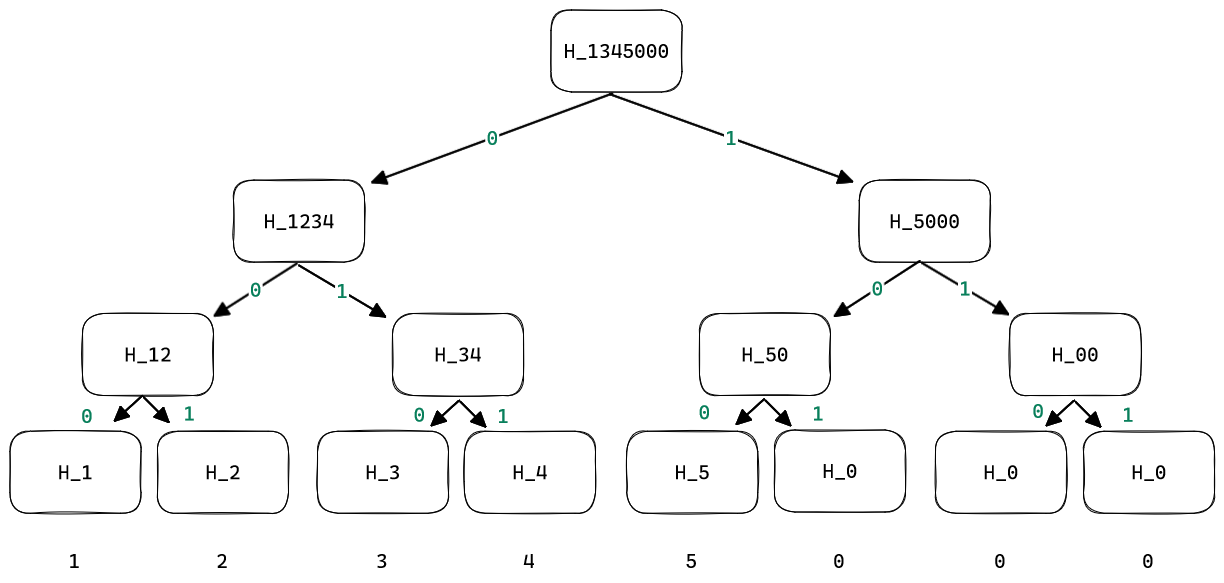
\includegraphics[width=13cm]{./chapters/2.rln-protocol/images/1.merkle_tree.png}
    \label{fig:merkle_tree}
    \captionsetup{justification=centering}
    \caption{Struttura albero di Merkle binario}
\end{figure}
Possiamo notare che la radice degli alberi di Merkle possiede la proprietà di essere una sorta di impronta digitale
della struttura, in quanto qualsiasi modifica ai dati comporterebbe un cambiamento a cascata dei nodi fino alla radice
stessa. Questa proprietà costituisce un vantaggio significativo in termini di efficienza. Infatti, consente una verifica
rapida delle modifiche apportate alla struttura, rendendo gli alberi di Merkle estremamente utili nei campi
decentralizzati e nei file system condivisi, dove l'individuazione efficiente dei cambiamenti con poche informazioni è
cruciale. Un'altra proprietà altamente utile degli alberi di Merkle è la loro capacità di verificare l'appartenenza di
un elemento alla struttura in modo efficiente e senza la necessità di conoscere l'elemento in chiaro. Nell'esempio
precedente, se si desidera verificare che l'elemento 4 appartenga alla struttura, è sufficiente utilizzare gli elementi
H\_3, H\_12 e H\_5000 e il valore H\_4, che non rivela alcuna informazione su l'elemento. Una volta ottenuta la radice
basterà confrontarla con la radice corretta per convincersi della presenza dell'elemento o meno nella struttura.
\begin{figure}[H]
    \centering
    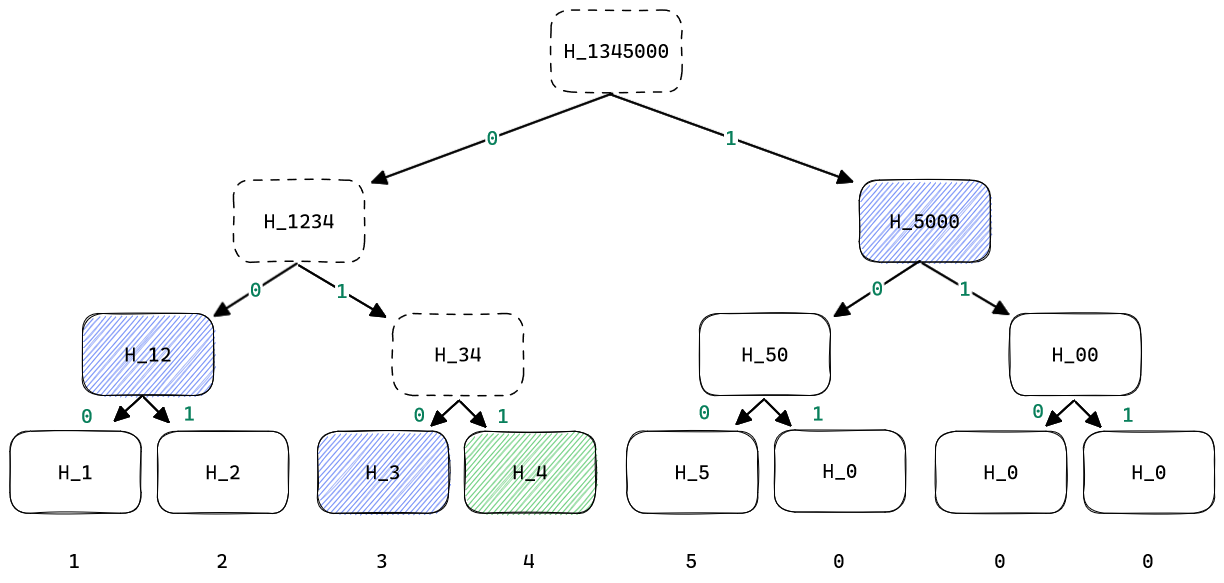
\includegraphics[width=14cm]{./chapters/2.rln-protocol/images/2.merkle_proof.png}
    \label{fig:merkle_proof}
    \captionsetup{justification=centering}
    \caption{Merkle proof}
\end{figure}
Questo processo viene chiamato "Merkle proof" o più in generale "proof of membership". Tale processo rappresenta
l'approccio che adotteremo per dimostrare la capacità di un utente già registrato e non rimosso di interagire con il
sistema nella fase di Interazione del protocollo RLN.

\subsection{Nuove funzioni di hash}
Indubbiamente, una delle tecniche più utilizzate in crittografia sono le funzioni di hash. Anche la tecnologia zk-SNARK
non può fare a meno di esse. Infatti, come abbiamo già visto in molte situazioni, l'utilizzo di metodi di hashing è
stato necessario per ridurre le dimensioni delle informazioni e per nasconderle. Tuttavia, quando si utilizzano le
tradizionali funzioni di hash come la versione Sha-256 nel campo delle Zero Knowledge proof, si verifica un problema.
Queste funzioni non sono state concepite per lavorare in domini di campi finiti e, pertanto, sfruttano metodologie come
la ripetizione di operazioni bit-wise, che tendono se trasformate con R1CS ad aumentare considerevolmente la dimensione
dei vincoli del circuito. Questo aumenta notevolmente il tempo e la dimensione richiesti
per generare le prove. Negli ultimi anni, per superare il problema descritto, sono state utilizzate nuove versioni di
funzioni hash come Pedersen, Rescue-$x^5$ e Poseidon. Queste funzioni sono state progettate specificamente per lavorare nei
campi finiti e con l'obiettivo di ridurre al minimo i tempi di generazione e i vincoli necessari per costruire le prove.
Tra queste funzioni, la funzione Poseidon è quella che ha ottenuto i risultati migliori e che verrà utilizzata nella
costruzione del circuito per il protocollo RLN. Di seguito vengono mostrate delle tabelle contenenti un confronto delle
prestazioni tra le più note funzione di hash per le tecnologie Zero Knowledge e la funzione Sha-256, tabelle tratte da
"POSEIDON: A New hash Function for Zero-Knowledge Proof Systems" \cite{cryptoeprint:2019-458}. Nelle tabelle sottostanti
possiamo notare che ci sono diverse configurazioni della funzione Poseidon. Infatti, una grande differenza tra le
funzioni tradizionali e Poseidon è la possibilità di scegliere il numero di iterazioni e la dimensione del campo finito
su cui lavorare, in modo da selezionare la versione più performante a seconda del caso.\\
\begin{figure}[H]
    \centering
    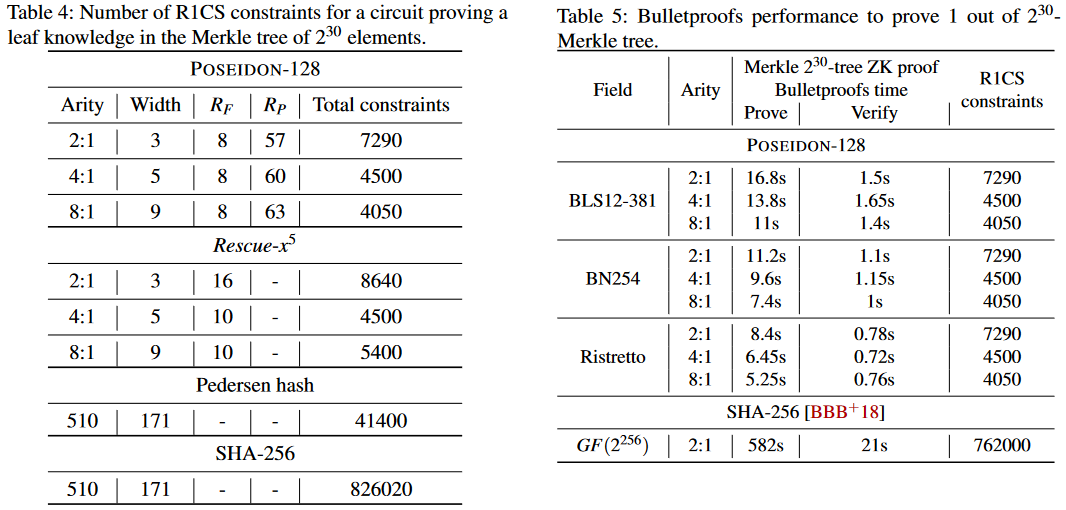
\includegraphics[width=14cm]{./chapters/2.rln-protocol/images/3.poseidon_comparison.png}
    \label{fig:poseidon_comparison}
    \captionsetup{justification=centering}
    \caption{Confronto algoritmi di hash, tratto da \cite{cryptoeprint:2019-458}}
\end{figure}

\subsection{Nullifier}
I "nullifier" in crittografia sono dei valori utilizzati per confermare o annullare operazioni. Nelle applicazioni che garantiscono
l'anonimato, questi valori vengono spesso utilizzati per evitare il problema del "double-signaling", ovvero impedire che
un utente utilizzi o esegua un'operazione che dovrebbe essere unica per ogni utente più di una volta. Questo problema
può verificarsi perché, in assenza di un collegamento tra i dati e le identità degli utenti, non è possibile verificare
se un utente ha già effettuato o completato una determinata operazione. Ad esempio, in un'applicazione elettorale è
importante impedire che un singolo elettore, voti più di una volta, mentre nel campo delle criptovalute è fondamentale evitare che la
stessa moneta, venga spesa più volte. Il problema si risolve utilizzando i nullifier ovvero valori univoci legati
all'operazione che rimangono privati fino al momento dell'effettuazione dell'operazione e una volta attuata vengono
resi pubblici, e salvati in modo da poterli consultare successivamente.
\begin{figure}[H]
    \centering
    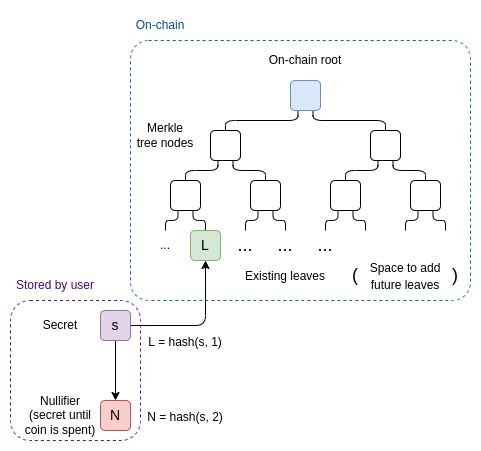
\includegraphics[width=10cm]{./chapters/2.rln-protocol/images/4.nullifier.png}
    \label{fig:nullifier}
    \captionsetup{justification=centering}
    \caption{Esempio Nullifier, tratta da \cite{some-ways-to-use-zk-snarks-for-privacy}}
\end{figure}
Dalla descrizione fornita potrebbe subito venire in mente il concetto di "rate-limiting" e si potrebbe pensate di
utilizzare i nullifier per attuare questa procedura in modo anonimo. In effetti, è possibile limitare gli
utenti utilizzando questa metodologia, però non si potrà rivelare l'identità dell'utente malintenzionato che, in questo
modo, potrebbe riprovare indisturbato ad attaccare il sistema.
\section{Registrazione}
La registrazione consiste nella prima fase del protocollo RLN, in questa fase gli utenti, previa la generazione di una chiave privata e ricavando da questa un "identity commitment" utilizzando la funzione hash Poseidon. Per semplificare la spiegazione da qui in poi, utilizzeremo il simbolo $a_0$ per indicare la chiave privata.
$$identityCommitment = Poseidon(a_0)$$
in alcuni casi potremmo avere la necessità di elaborare maggiormente la creazione dell'identity commitment per aumentare il livello di sicurezza o associare all'identity commitment anche una stake. Una volta generato l'identity commitment l'utente viene inserito all'interno del albero di Merkel del sistema. A questo punto l'utente sarà in grado di generare dell "proof of membership" e quindi di interrogare il sisteam. Per evitare attacchi di tipo Sybil, è posibile implementare dell'tecniche che vincolino l'inserimento dell'utente nell albero al rispetto di alcuni vincoli, come posseso identità digitali o di un profilo social accreditato o ancora un portafolgio di criptovalute.

Tra i progetti del gruppo PSE troviamo anche un progetto chiamato Interep, il cui scopo è essenzialemtene estrapolare la reputazione di un utente e inserire un identity commitment a lui associato all'inetrno di alcuni gruppi di reputazione. Questi gruppi (alberi di Merkel) sono divisi in base al grado di reputazione degli utenti. Attualemente il progetto Iterep permette di estrapolare la reputazione di un utente dagli acocunt socail di Github, Twitter e Reddit.
\section{Interazione}
Passata la fase di registrazione, gli utenti avranno la possibilità di effettuare richieste. Ora ci chiediamo come possaimo implementare una regola di rate-limiting del tipo: "Un utente non può fare più di $k$ richieste per un determinato lasso di tempo $e$ (epoca)"?

RLN utilizza l'algoritmo Shamir's Secret Sharing (SSS) che permette di suddividere un segreto in $n$ parti in cui ciascuna parte del segreto non rivela nulla, ma se ne vengono combinate $k$ dove $k < n$ allora il segreto può essere ricostruito. Ogni volta che l'utente fa una richiesta al sistema, rilascia una delle $n$ porzioni in cui la sua chiave privata $a_0$ è stata divisa. In questo modo, se l'utente raggiungesse il valore di soglia $k$ imposto dalla regola di rate limiting il sistema sarebbe in grado di ricostruire $a_0$ svelando l'identità dell'utente.

La procedura per dividere e ricostruire il segreto si basa ancora una volta sull'utilizzo di polinomi, in particolare sull'interpolazione di Lagrange. Il grado del polinomio da utilizzare per ricostruire la chiave privata a partire dai suoi componenti dipende strettamente dal numero di richieste che si desidera consentire. In particolare, per interpolare (cioè ricostruire) un polinomio di grado $k$, abbiamo bisogno di almeno $k+1$ punti.

Per consolidare il tutto vediamo un esempio. immaginiamo di voler applicare una regola di rate limiting in cui :
"Un utente non può fare più di 1 richiesta al minuto". 

Per prima cosa costruiamo un nullifier, che ci servirà per identificare i messaggi inviati all'interno di un epoca:
$$externalNullifier = Poseidon(epoch,rln\_identifier)$$
dove $epoch$ è l'epoca in cui è stato invito il messaggio e $rln\_identifier$ è un valore univoco per tutta l'applicazione che utilizza il protocollo. Poi proseguiamo costruendo il polinomio che dovrà essere ricostruito dal verificatore (il sitema), costruiamo il polinomio in modo che con due richieste ovvero due punti sia possibile ricostruire il segreto, quindi usiamo un poilinomio di primo grado costruito come segue:
$$ A(x) = a_1 * x + a_0$$
possaimo notare che il polinomio valutato in 0 vale $a_0$ la nostra chiave privata, mentre $a_1$ è definito come $a_1 = Poseidon(a_0, externalNullifier)$ e permette di variare il polinomio in base all'epoca in cui viene fatta la richietsa. Quando un utente invia una richiesta al sistema calcola anche due coordinate $x = Poseidon(richiesta)$ e ottenendo $y=A(x)$ che identificano una porzione delle segreto ovvero un punto sul polinomio. Se un utente malitenzionato inviasse un altro messagio con le nuove coordinate $x_2 = Poseidon(richiseta_2)$ e $y_2=A(x_2)$ nella setessa epoca (ovvero con lo stesso polinommio) il sitema sarebbe in grado di ricostruire il polinomio interpolando i due punti. Nel caso di polinomio di primo grado questa procedura è immediata
\begin{figure}[H]
    \centering
    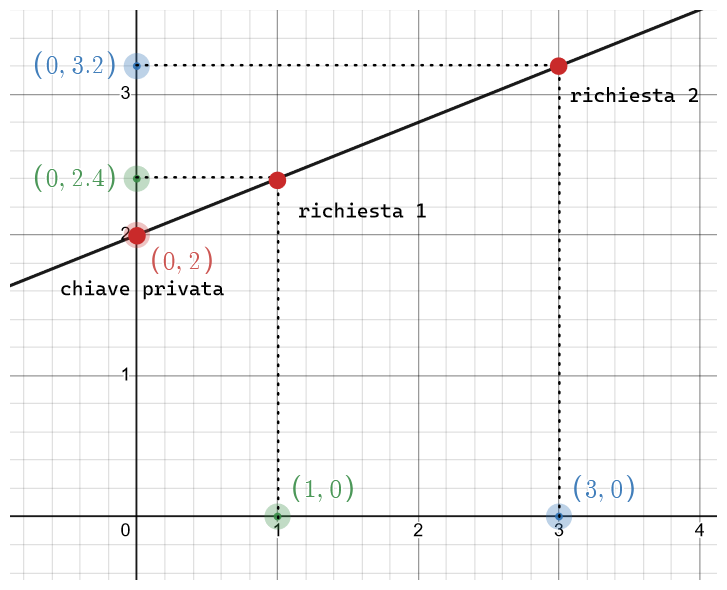
\includegraphics[width=11cm]{./chapters/2.rln-protocol/images/6.a_0_interpolation.png}
    \label{fig:a_0_interpolation}
    \captionsetup{justification=centering}
    \caption{Grafico SSS pilinomio primo grado}
\end{figure}
RLN utilizza l'algoritmo Shamir's Secret Sharing (SSS) che permette di suddividere un segreto in $n$ parti in cui ciascuna parte del segreto non rivela nulla, ma se ne vengono combinate $k$ dove $k < n$ allora il segreto può essere ricostruito. l'algoritmo SSS utilizza l'interpolazione di lagrange per  Per compredere il tutto riportamoci ad un esempio immaginiamo di voler implementare una regola del tipo "Un utente non deve poter effettuare più di 1 richiesta al minuto"
\section{Punizione}
L'ultima fase del protocollo consiste nella punizione dell'utente malintenzionato. Questa procedura è fortemente legata
al contesto applicativo. L'idea generale è che se sono presenti $k$ porzioni diverse per ricostruire
$a_0$ dalle coordinate $x$ e $y$, allora l'identità dell'utente può essere rivelata e l'utente può essere rimosso
dall'albero di Merkle ricostruendo il suo l'identity commitment. Questo comporta
l'azzeramento della foglia che contiene l'identity commitment dell'utente all'interno dell'albero. Inoltre, a seconda dell'applicazione,
la chiave privata può anche essere usata per sequestrare la stake fornita dall'utente.

\chapter*{Prototipo}
\chaptermark{Prototipo}
\addcontentsline{toc}{chapter}{Prototipo}

In questo capitolo, presenteremo le parti significative di un prototipo di applicazione che utilizza il protocollo RLN e la tecnologia zk\_SNARK  per applicare una regola di limitazione della velocità in un sistema centralizzato, dove Client e Server interagiscono in completo anonimato.

Al fine di concentrarci sulle dinamiche del protocollo per comprenderne il funzionamento, ho scelto di semplificare la parte strutturale del prototipo, che è composta da un Server che espone un servizio di registrazione e di interazione, e alcuni Client che comunicano con il Server attraverso un canale di comunicazione basato su socket.

Si tenga presente che il protocollo non ha pretese di essere un progetto realmente funzionante, ma piuttosto di essere un utile strumento per coloro che desiderano acquisire familiarità con le tecnologie zero knowledge e applicarle concretamente. Ciò nonostante sarà possibile valutare i benefici e le criticità che queste tecnologie portano in campo, mediante il calcolo delle prestazioni e l'analisi del codice.

\section{Tecnologie e struttura}
Per lo sviluppo del prototipo, ho attuato la scelta di utilizzare il linguaggio di programmazione TypeScript. Questa decisione è stata presa in considerazione delle specifiche necessità del progetto, e in particolare delle librerie sviluppate e attive per la tecnologia zk-SNARK e per il protocollo RLN. La struttura del progetto è un monorepo (unica repository con molteplici progetti) che contiene sia i dati e il codice del Server che quelli reltiva al Client. Entrambi i componenti, utilizzano Node.js come ambiente di esecuzione. Infatti dopo la compilazione del codice TypeScript in JavaScript, il codice viene eseguito tramite il runtime Node.js. 
Le librerie utilizzate sono le seguenti:
\begin{itemize}
    \item \textbf{Circom 2}: usata per la generazione e la compilazione dei circuiti del progetto. Circom consiste di un compilatore Rust per i circuiti scritti l'inguaggio circom (omonimo della libreria). Inotre comprende anche diversi template di circuiti che assolvono specifiche funzioni molto utli come l'implementazione della funzione di hash Poseidon.
    \item \textbf{Socket.IO}: è una libreria JavaScript che consente di creare e gestire connessioni in tempo reale tra il Client e il Server. Si basa sul protocollo WebSocket e permette di creare una comunicazione bidirezionale tra il Client e il Server implementando anche un sistema basato sugli eventi, ispirato alla classe EventEmitter di Node.js
    \item \textbf{RLN Circuits}: in questa libreria sono preseti i circuiti che implementano le funioni principarli del protocollo RLN. In particolare, sono presenti i circuiti per la registrazione, la verifica, la punizione e alcuni circuiti di supporto.
    \item \textbf{RLNjs}: è una libreria scritta in TypeScript che implementa la logica del protocollo RLN. Sfrutta i circuiti messi a disposizione dalla libreria precedente per implementare la logica di verifica e generazione delle prove.
\end{itemize}

Inoltre ho utilizzato il package manager ufficiale di Node.js, npm, per installare rapidamente e facilmente le librerie e i moduli di cui hai avuto bisogno e Eslint uno strumento di analisi del codice statico che aiuta a individuare e correggere errori e eventuali vulnerabilità del codice.

\section{Circuiti}
Come spiegato nella sezione relativa alla proprietà succint di zk-SNARK per potre creare un programma che usi questa tecnologia, abbiamo bisogno di formulare le porzioni di logica del programma che vogliamo provare (dimostrare) attraverso dei circuiti algebrici. Le parti significative del codice di cui vogliamo creare una Zero Knowledge Proof sono l'appartenzenza all'albero di Merkle e la corretta costruzione delle porzione di segreto che ogni Client rilascia al Server durante l'interazione. Per questo motivo abbiamo bisogno di due circuiti:
\begin{enumerate}
    \item \textbf{proof of membership}:
    \begin{figure}[H]
        \centering
        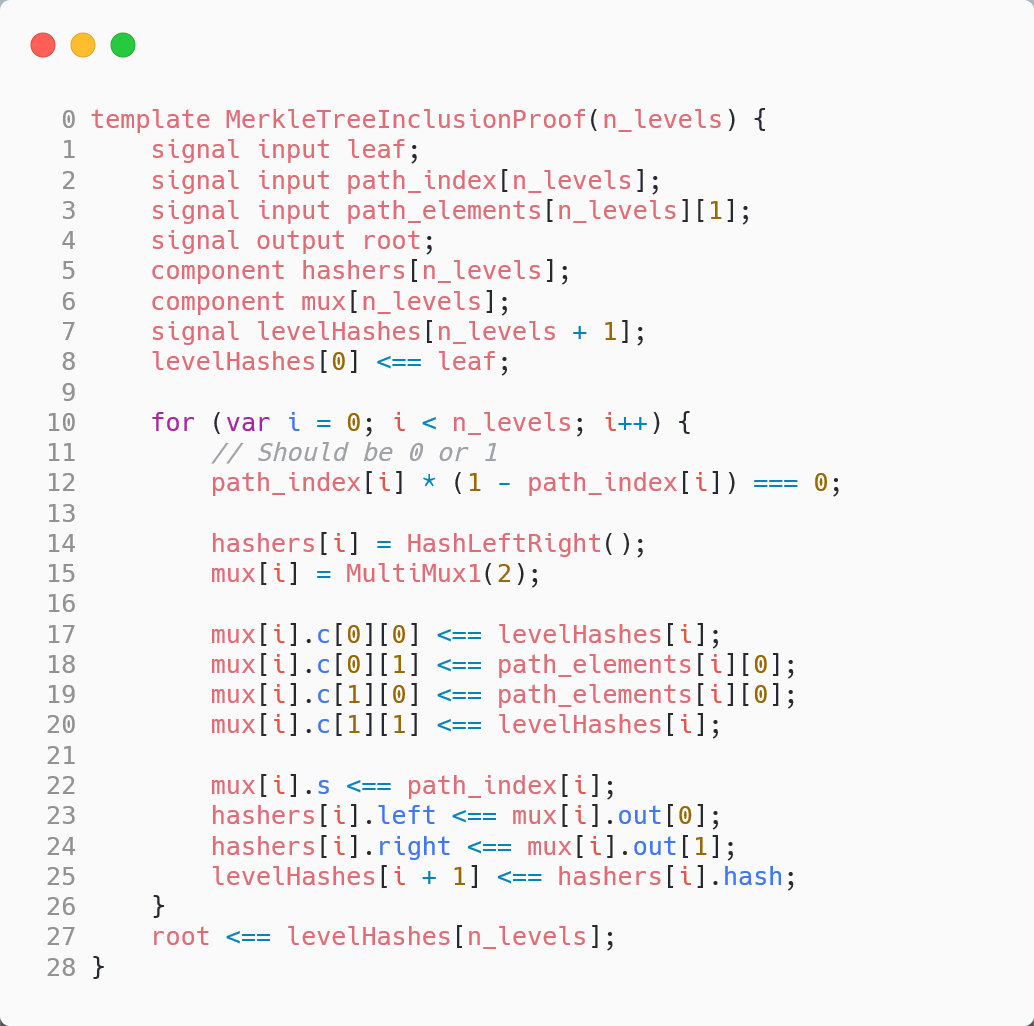
\includegraphics[width=10cm]{./chapters/3.poc/images/1.merkle_proof.png}
        \label{fig:merkle_proof}
        \captionsetup{justification=centering}
        \caption{codice circuito proof of membership}
    \end{figure}
    Nel codice in figura possiamo vedere il circuito scritto in codice circom che implementa la ricerca di un elemento all'interno di un albro di Merkle, il circuito prende in ingresso tre paramentri: la prfonditò dell' albero, il valore della foglia da cercare, il percorso binario, dove 0 indica il ramo di sinistra e 1 indica il ramo di destra, che bisogna seguire partendo dalla radice per raggiungere la foglia e le altre foglie dell'albero. Il circuito restiturisce la radice dell'albero. I componenti $HashLeftRight()$ e $MultiMux1()$ sono due componenti ausiliari che servono rispettivamente a apllicare la funzione hash ai nodi figli e a selezionare i nodi corretti in base al livello dell'albero in cui ci troviamo.
    \item \textbf{verifica delle porzioni del segreto}:
    \begin{figure}[H]
        \centering
        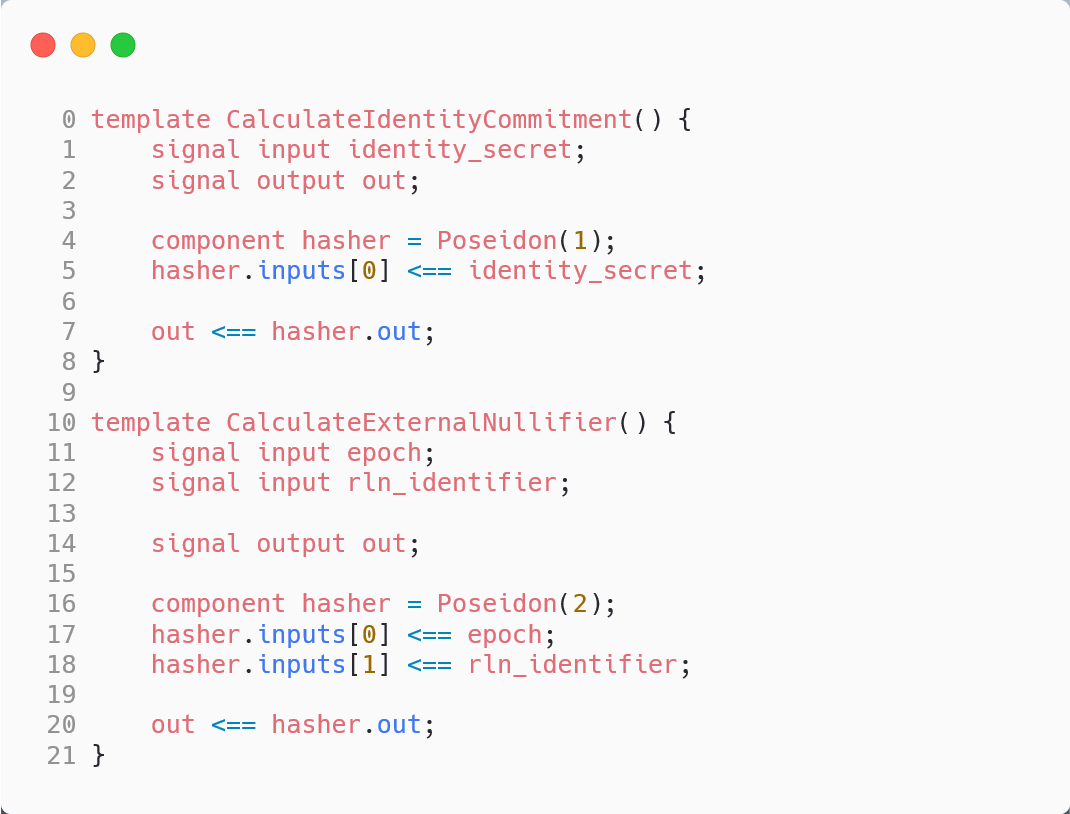
\includegraphics[width=11cm]{./chapters/3.poc/images/2.1.verify_shares.png}
        \label{fig:1.verify_shares}
        \captionsetup{justification=centering}
        \caption{codice circuito proof of membership}
    \end{figure}
    In questa prima porzione di codice possiamo vedere due funzioni fondamentali del protocollo RLN, ovvero la funzione $CalculateIdentityCommitment()$ che permette di verificare che l'identity commitment venga effettivamente calcolato a partire dalla chiave privata e $CalculateExternalNullifier()$ che è quel circuito ci permette di ottenere un nullifiere diverso per singolo mesaggio.\clearpage
    \begin{figure}[H]
        \centering
        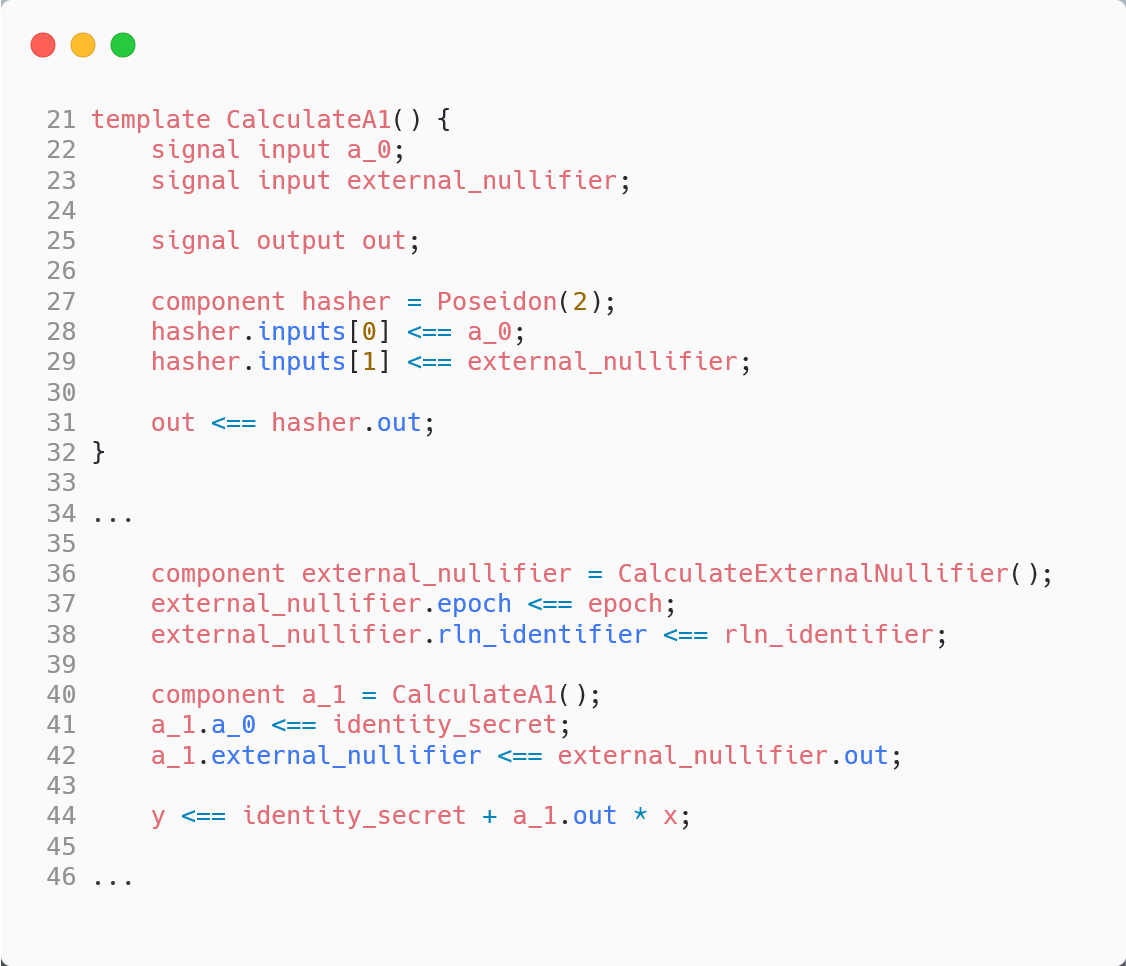
\includegraphics[width=11cm]{./chapters/3.poc/images/2.2.verify_shares.png}
        \label{fig:2.verify_shares}
        \captionsetup{justification=centering}
        \caption{codice circuito proof of membership}
    \end{figure}
    Mentre in questa porzione vediamo ancora una funzione atomica ovvero CalculateA1() che permette di ottenere il valore a1 che fa variare il polinomio di verifica a seconda dell' external\_nullifier e della chiave privata seguendo la formula vista in precedenza $a_1 = Poseidon(a_0, externalNullifier)$ e in fine vediamo una porzione di codice dove tutte le funzioni precedenti vengono utilizzate per verificare che il segreto sia stato costruito correttamente.
\end{enumerate}

Ricordo che il codice visto fino ad adesso non rappresenta la logica del protocollo ma solamente, i circuiti algebrici che verranno trasformati in vincoli per la verifica che il Client soddisfi e rispetti pur rimanendo anonimo le regole del servizio.

Per ottenere i file che verranno utilizzati da Server e Client per provare e verificare le dimostazione, bisogna compilare i circuiti utilizzando circom. Alla fine della fase di compilazione che si divide in trasformazione da circuito a QAP e successiva fase di trustedSetup che ovviamente in questo caso è stat svolta con un unico partecipantem, otteniamo i seguenti file:
\begin{itemize}
    \item \textbf{rln\_final.zkey}: file che contiene i parametri crittografici e i paramentri privati che consentono a un verificatore di controllare la validità di una prova senza rivelare alcuna informazione sui dati sottostanti.
    \item \textbf{rln.wasm}: è una versione compilata del circuito che può essere eseguita in un browser web utilizzando WebAssembly. Questo file è generato dal codice Circom e contiene la logica del circuito in un formato binario che può essere eseguito.
    \item \textbf{verification\_key.json}: contiene una chiave pubblica relativa al circuito, che può essere usata da un verificatore per controllare la validità di una prova.
\end{itemize}

\section{Server}
La struttura del Server è semplice: si tratta di un progetto Node.js che utilizza la libreria Socket.IO per gestire la comunicazione con i Client. Il Server è composto da due classi principali: "server.ts" e "type.ts". La prima classe contiene la logica applicativa e implementa le primitive della libreria RLNjs per verificare le prove dei Client. La seconda classe è un file che definisce degli enum, utilizzati per identificare lo stato e gli eventi di comunicazione tra il Server e i Client. Questo file, insieme ai file di configurazione del circuito, è presente sia nel progetto Server che in quello Client.

Il Server attende la comunicazione con un Client sulla porta 3000 e rimane in attesa fino a quando non riceve un evento. Gli eventi possibili sono definiti nel file "type.ts" e quelli accettati dal Server sono EventType.REGISTER e EventType.INTERACTION. Questi eventi sono utilizzati rispettivamente per gestire la registrazione e l'interazione con gli utenti. Durante la fase di registrazione, il Server inserisce gli utenti nell'albero di Merkle, chiamato "registry" nel programma, e notifica lo stato della registrazione, che può essere uno dei seguenti: ALREADY\_REGISTERED, BANNED o VALID. 
\begin{figure}[H]
    \centering
    \includegraphics[width=10cm]{./chapters/3.poc/images/3.1.Server.png}
    \label{fig:1.Server}
    \captionsetup{justification=centering}
    \caption{codice Server gestione registrazione}
\end{figure}
Mentre per quanto riguarda la fase di interazione, il Server si occupa prima di tutto di controllare che l'utente abbia inviato una prova valida. Questo controllo avviene verificando che la radice del suo registry collimi con quella del Server e che la generazione della prova abbia seguito i vincoli specificati dal circuito. Successivamente, il Server controlla se il messaggio inviato rispetta le regole anti-spam. Se ciò non avviene, il Server rimuove l'utente e sincronizza i registry dei suoi Client inviando un messaggio di broadcast a tutti i membri. Nelle fasi successive, approfondiremo i tempi necessari per lo svolgimento di queste funzioni.
\begin{figure}[H]
    \centering
    \includegraphics[width=10cm]{./chapters/3.poc/images/3.2.Server.png}
    \label{fig:2.Server}
    \captionsetup{justification=centering}
    \caption{codice Server gestione interazione}
\end{figure}

\section{Client}
Il Client presenta una struttura molto simile a quella del server, utilizza la libreria Socket.IO-client per gestire la comunicazione. Inoltre, dispone di un file "type.ts" analogo a quello del server per gestire gli eventi di comunicazione e conserva all'interno del progetto i file relativi alla generazione del circuito. Tuttavia, a differenza del server, il Client utilizza tali file per generare le prove e non per verificarle. Gli eventi rilevanti per il Client sono EventType.REGISTER, EventType.INTERACTION, EventType.USER\_REGISTERED e EventType.USER\_SLASHED. Gli ultimi due sono generati dal Server e servono a sincronizzare gli alberi di merkle degli utenti a seguito della registrazione o rimozione di un nuovo membro, infatti per poter generare prove valide, gli utenti devono possedere la stessa versione della struttura posseduta dal Server altrimenti il primo controllo sulla radice dei registri, non andrebbe a buon fine. \clearpage
\begin{figure}[H]
    \centering
    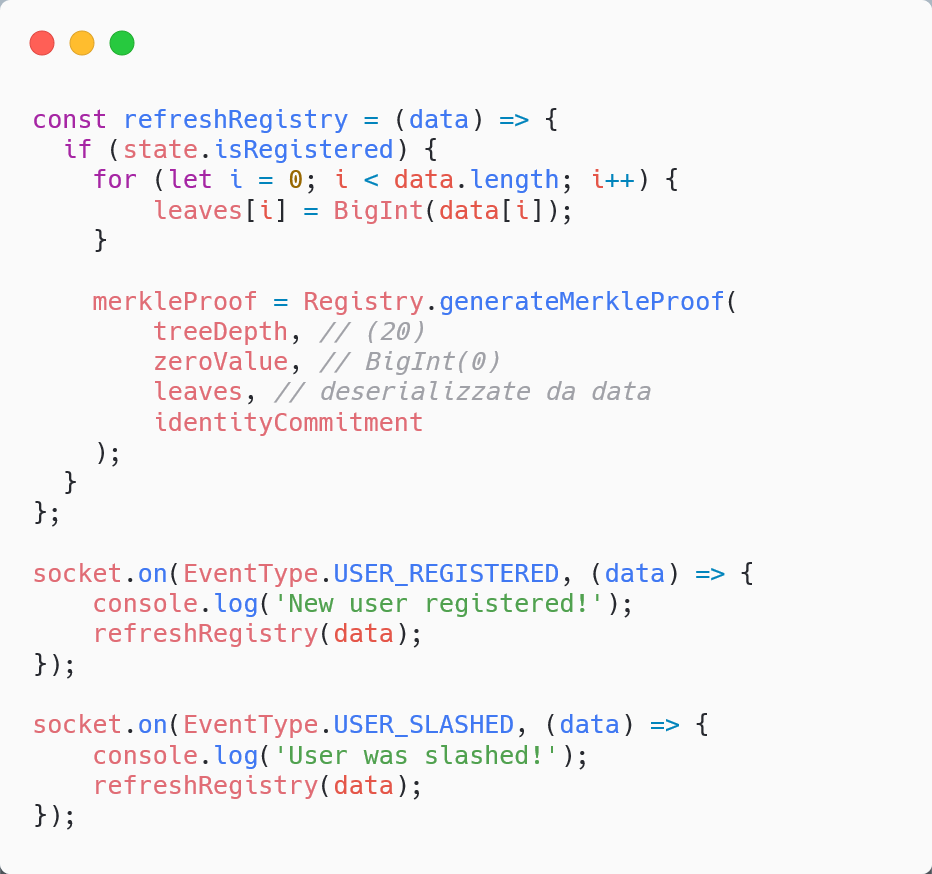
\includegraphics[width=10cm]{./chapters/3.poc/images/4.1.client.png}
    \label{fig:1.client}
    \captionsetup{justification=centering}
    \caption{codice Client sincronizzazione registri}
\end{figure}
Per ottimizzare la fase di interazione la generazione della prova di appartenenza al registro viene effettuata ad ogni sincronizzazione.
La fase di registrazione è abbastanza banale in quanto è costituita solamente dall'invio dell'identity commitment al server a dall'attesa del relativo aknowledgement. Mentre la fase di interazione è più articolata in quanto è durante questa fase che il Client genera la prova di appartenere all'albero e di avere generato le porzioni di chiave da rilascaire in modo corretto. In questa fase, per testare le funzionalità di rate limiting, ho incluso la possibilità per l'utente di selezionare l'opzione "dos". Grazie a questa opzione, l'utente potrà provare ad inviare 100 messaggi nello stesso intervallo di tempo. Prima d'interagire con il sistema l'utente genera una prova utilizzando il segnale, che una volta applicata la funzione hash rappresenterà la nostra cordinata $x$, la merkleProof e l'externalNullifier. Le altre infomazioni necessarie come la chiave privata o l'rln\_identifier vengono ricavate da un istanza della libreria RLNjs creata durante le fasi iniziali del Client.\clearpage
\begin{figure}[H]
    \centering
    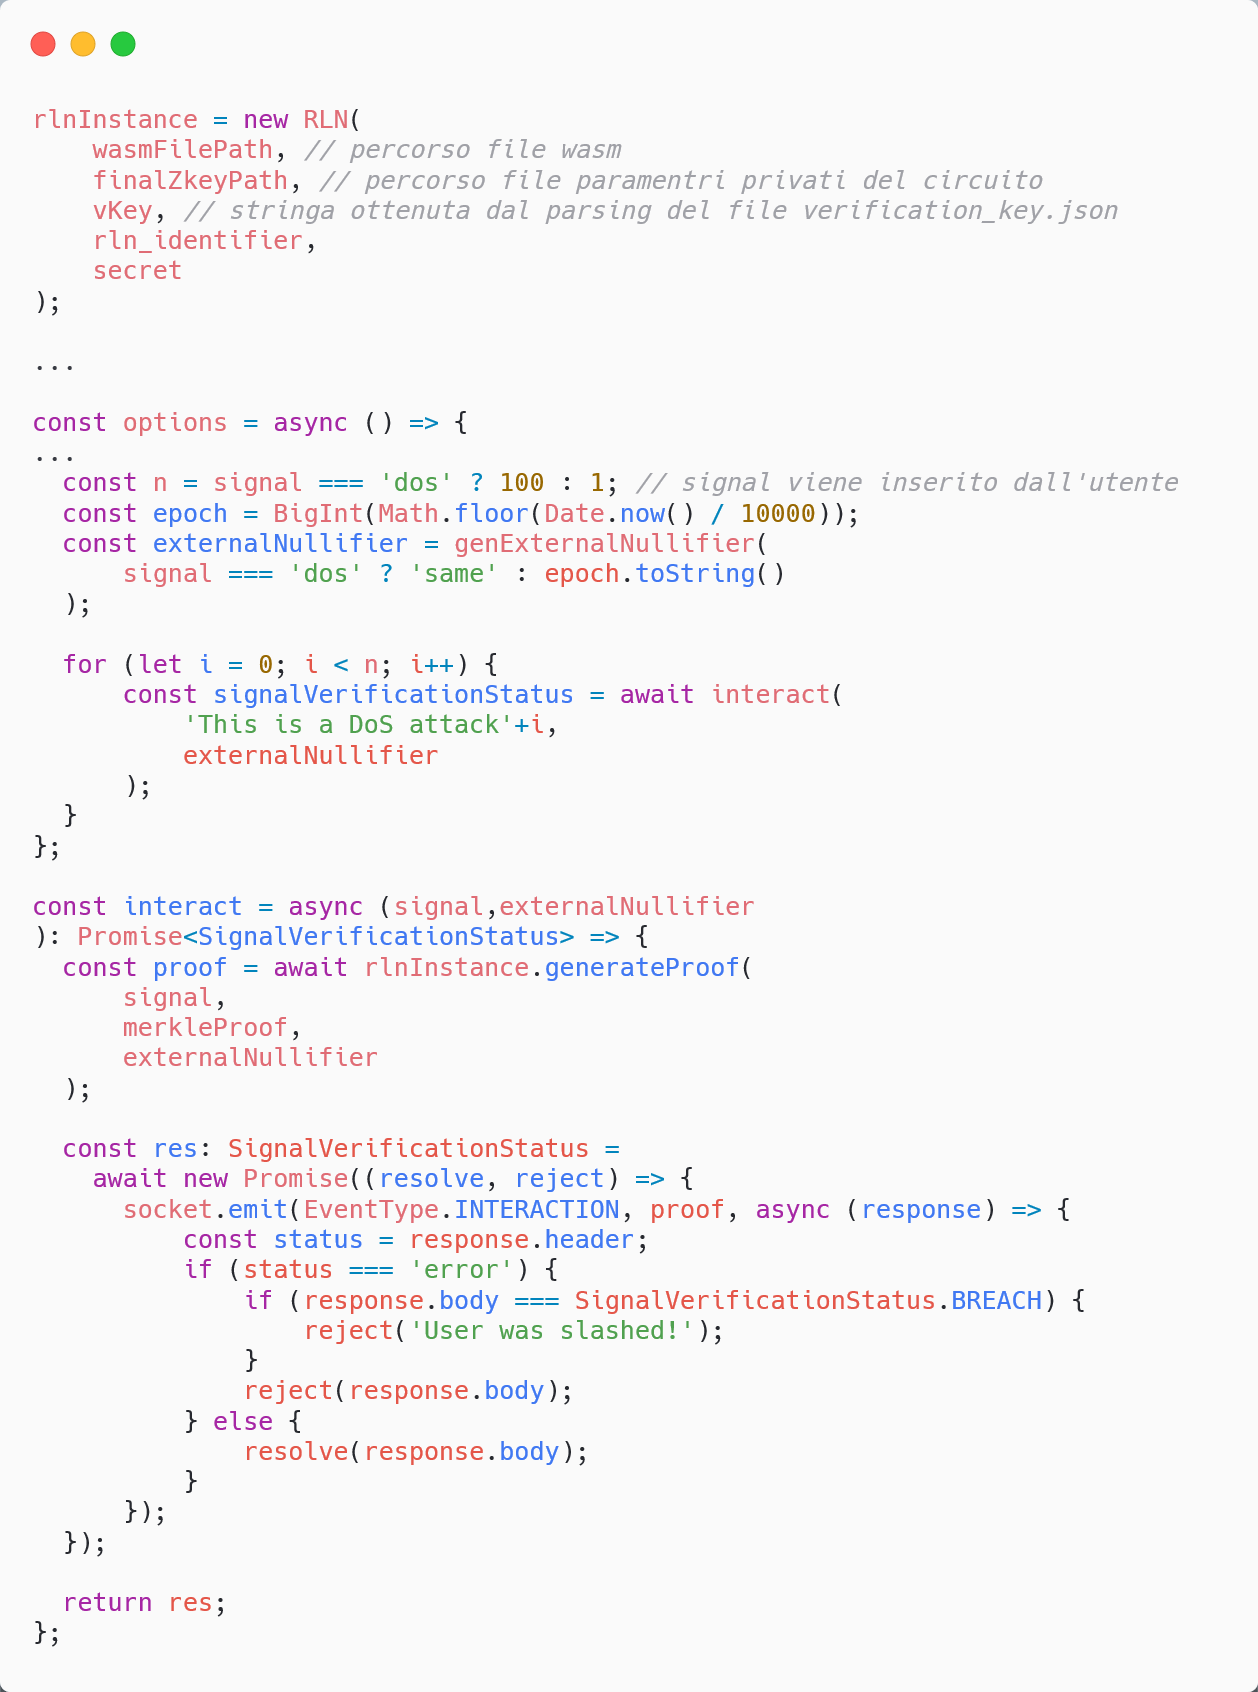
\includegraphics[width=11cm]{./chapters/3.poc/images/4.2.client.png}
    \label{fig:2.client}
    \captionsetup{justification=centering}
    \caption{codice Client interazione con il sistema}
\end{figure}

\section{Prestazioni}
Di seguito riporto alcuni dati significativi ottenuti dall'esecuzione del prototipo. I test sono stati effettuati su un computer con le seguenti caratteristiche:
\begin{itemize}
    \item CPU: Apple silicon M1
    \item RAM: 8GB
    \item OS: MacOS Ventura 13.0
\end{itemize}

Inizieremo analizzando il numero di vincoli che costituiscono i circuiti per la generazione delle prove e le loro dimensioni. È importante ricordare che i circuiti sono stati generati utilizzando la libreria Circom 2. Per i test che verranno presentati, sono state utilizzate tre diverse profondità degli alberi di Merkle: 16, 24 e 32, che corrispondono rispettivamente ad un massimo di $2^{16}$, $2^{24}$ e $2^{32}$ utenti.
\begin{figure}[H]
    \centering
    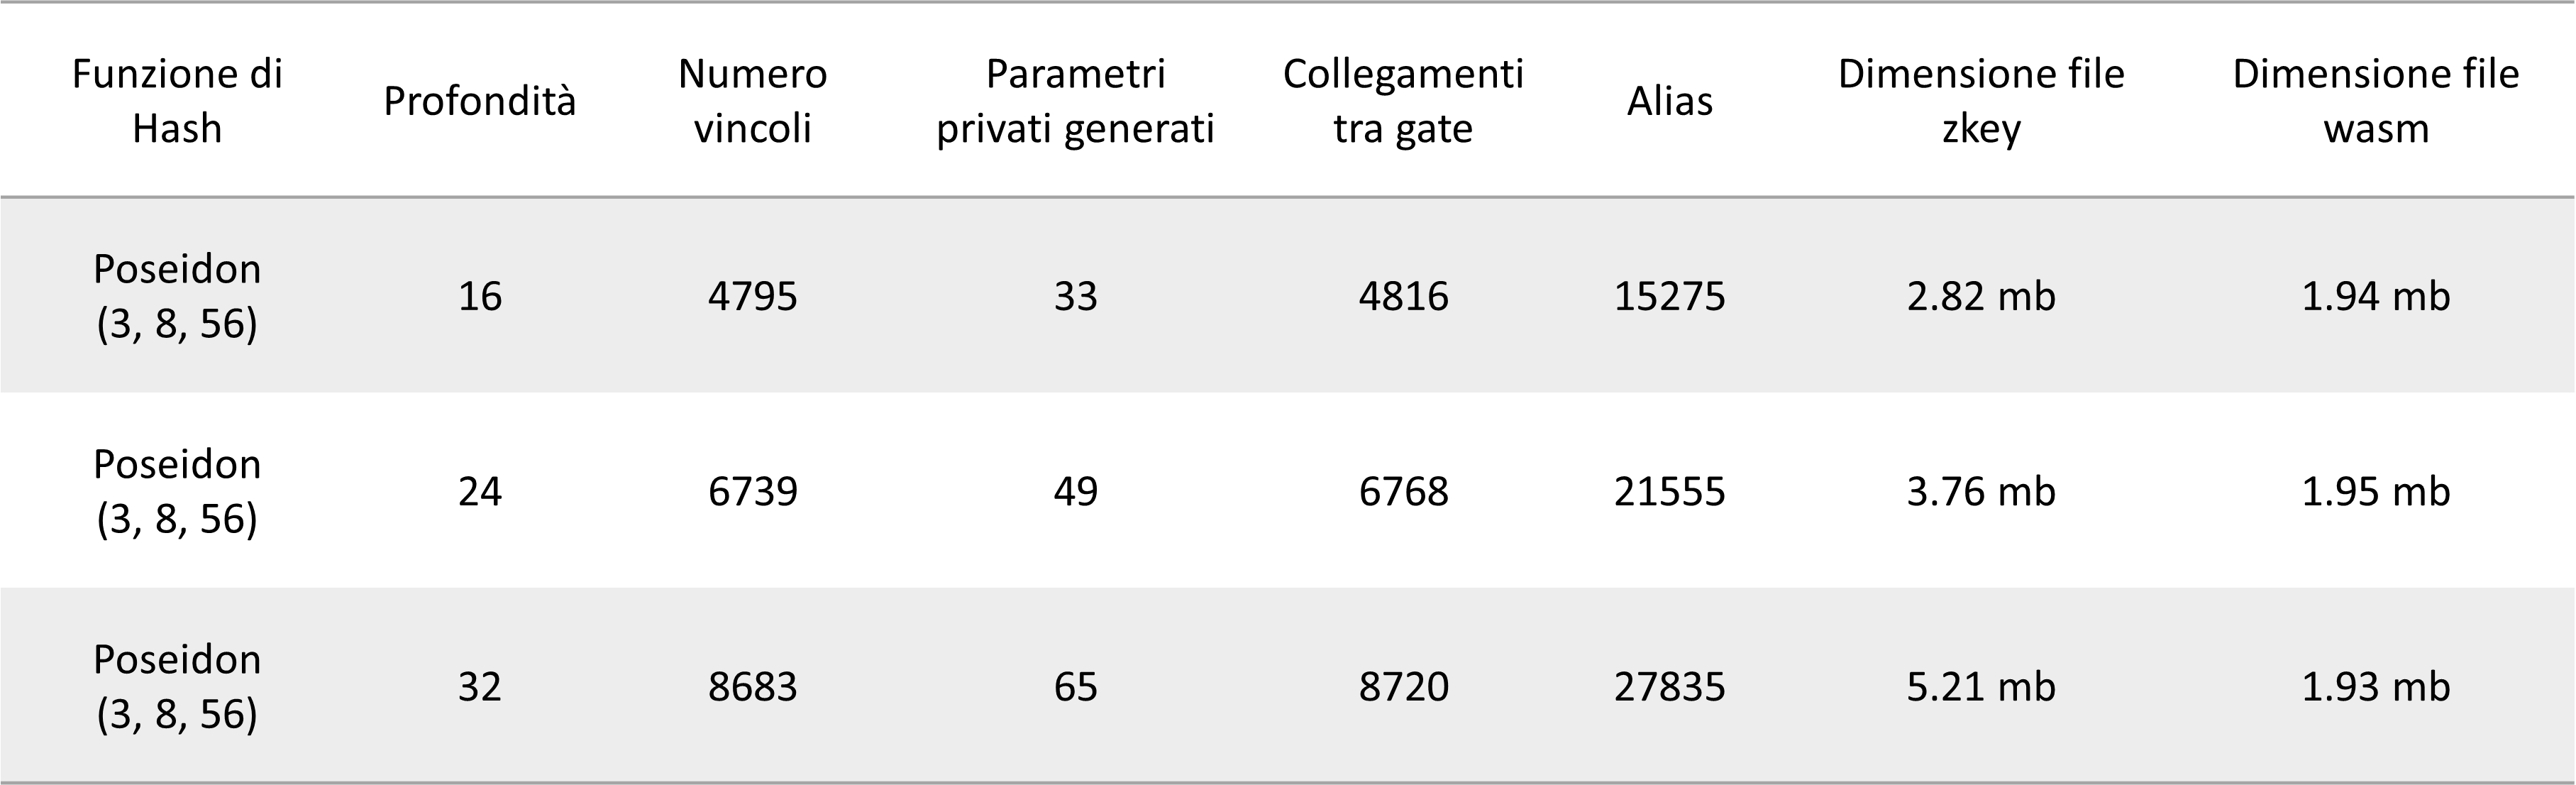
\includegraphics[width=17cm]{./chapters/3.poc/images/5.1.bench.png}
    \label{fig:1.bench}
    \captionsetup{justification=centering}
    \caption{codice Client interazione con il sistema}
\end{figure}
I dati più significativi sono il numero di vincoli, le dimensioni dei file rln\_final.zkey e rln.wasm. Infatti, se a un primo impatto i numeri dei vincoli generati dai circuiti possono sembrare molto elevati, in realtà le dimensioni dei file sono notevolemente ridotte, se pensiamo che un albero di Merkle di profondità 30 utilizzando una funzione di hash con output 128 bit, può arrivare pesare decine di GB. Di seguito invece mostriamo i tempi di esecuzione:
\begin{figure}[H]
    \centering
    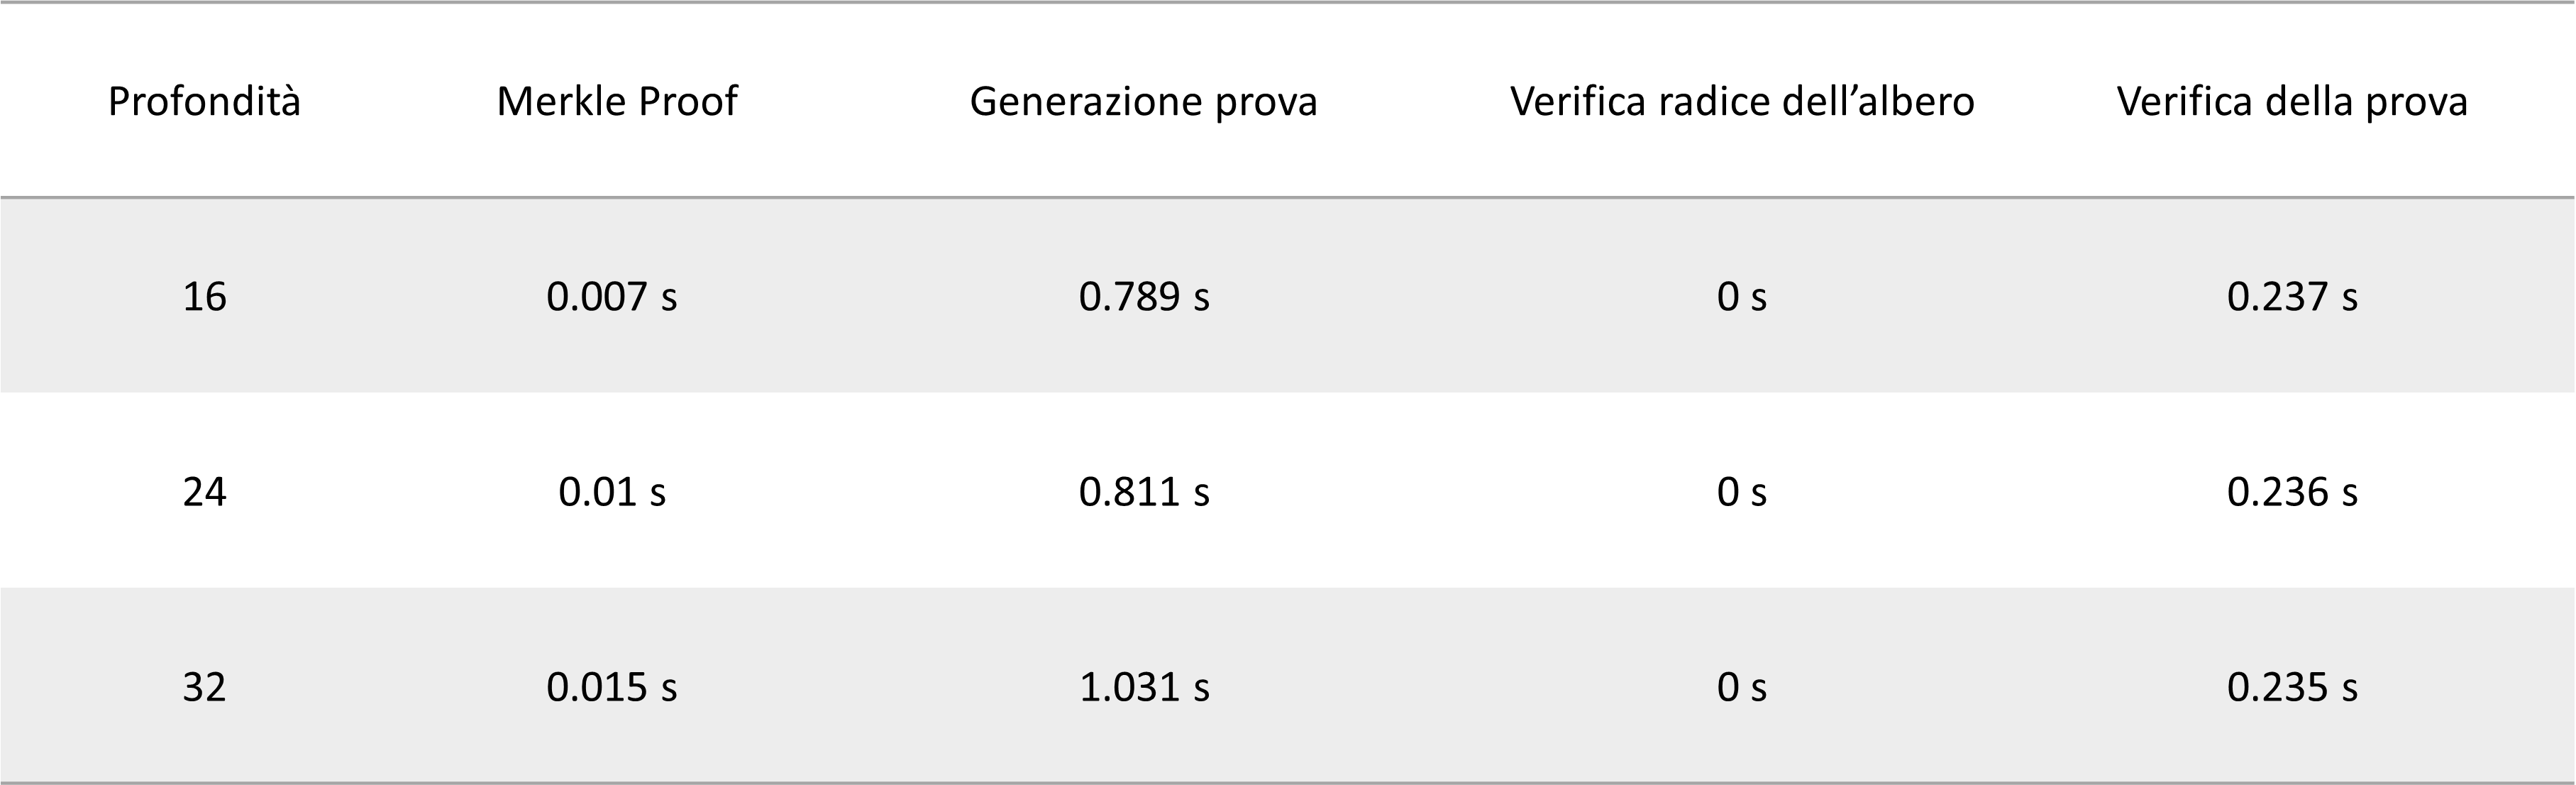
\includegraphics[width=17cm]{./chapters/3.poc/images/5.2.bench.png}
    \label{fig:2.bench}
    \captionsetup{justification=centering}
    \caption{codice Client interazione con il sistema}
\end{figure}

qui i dati più significativi sono i tempi di generazione e verifica delle prove, in particolare la verifica che rimane praticamente costante. La colonna con indice "Verifica radice dell'albero" rappresenta la velocità con cui il sistema riesce a verificare se la radice dell'albero con cui è stata generata la prova è uguale a quello correto.
\chapter*{Ringraziamenti}
\chaptermark{Ringraziamenti}
\addcontentsline{toc}{chapter}{Ringraziamenti}
Ringrazio i miei relatori per il supporto e per avermi dato l'opportunità di approfondire questa tema.

Altrettanto ringrazio i miei genitori e tutti coloro che mi sono stati vicini in questo percorso e hanno creduto in me.
A loro è dedicata questa tesi.

\printbibliography[heading=bibintoc]
\end{document}